% Options for packages loaded elsewhere
\PassOptionsToPackage{unicode}{hyperref}
\PassOptionsToPackage{hyphens}{url}
\PassOptionsToPackage{dvipsnames,svgnames,x11names}{xcolor}
%
\documentclass[
  a4paperpaper,
]{article}

\usepackage{amsmath,amssymb}
\usepackage{iftex}
\ifPDFTeX
  \usepackage[T1]{fontenc}
  \usepackage[utf8]{inputenc}
  \usepackage{textcomp} % provide euro and other symbols
\else % if luatex or xetex
  \ifXeTeX
    \usepackage{mathspec} % this also loads fontspec
  \else
    \usepackage{unicode-math} % this also loads fontspec
  \fi
  \defaultfontfeatures{Scale=MatchLowercase}
  \defaultfontfeatures[\rmfamily]{Ligatures=TeX,Scale=1}
\fi
\usepackage{lmodern}
\ifPDFTeX\else  
    % xetex/luatex font selection
\fi
% Use upquote if available, for straight quotes in verbatim environments
\IfFileExists{upquote.sty}{\usepackage{upquote}}{}
\IfFileExists{microtype.sty}{% use microtype if available
  \usepackage[]{microtype}
  \UseMicrotypeSet[protrusion]{basicmath} % disable protrusion for tt fonts
}{}
\makeatletter
\@ifundefined{KOMAClassName}{% if non-KOMA class
  \IfFileExists{parskip.sty}{%
    \usepackage{parskip}
  }{% else
    \setlength{\parindent}{0pt}
    \setlength{\parskip}{6pt plus 2pt minus 1pt}}
}{% if KOMA class
  \KOMAoptions{parskip=half}}
\makeatother
\usepackage{xcolor}
\usepackage[top=30mm,left=30mm,right=30mm,heightrounded]{geometry}
\setlength{\emergencystretch}{3em} % prevent overfull lines
\setcounter{secnumdepth}{-\maxdimen} % remove section numbering
% Make \paragraph and \subparagraph free-standing
\ifx\paragraph\undefined\else
  \let\oldparagraph\paragraph
  \renewcommand{\paragraph}[1]{\oldparagraph{#1}\mbox{}}
\fi
\ifx\subparagraph\undefined\else
  \let\oldsubparagraph\subparagraph
  \renewcommand{\subparagraph}[1]{\oldsubparagraph{#1}\mbox{}}
\fi

\usepackage{color}
\usepackage{fancyvrb}
\newcommand{\VerbBar}{|}
\newcommand{\VERB}{\Verb[commandchars=\\\{\}]}
\DefineVerbatimEnvironment{Highlighting}{Verbatim}{commandchars=\\\{\}}
% Add ',fontsize=\small' for more characters per line
\usepackage{framed}
\definecolor{shadecolor}{RGB}{241,243,245}
\newenvironment{Shaded}{\begin{snugshade}}{\end{snugshade}}
\newcommand{\AlertTok}[1]{\textcolor[rgb]{0.68,0.00,0.00}{#1}}
\newcommand{\AnnotationTok}[1]{\textcolor[rgb]{0.37,0.37,0.37}{#1}}
\newcommand{\AttributeTok}[1]{\textcolor[rgb]{0.40,0.45,0.13}{#1}}
\newcommand{\BaseNTok}[1]{\textcolor[rgb]{0.68,0.00,0.00}{#1}}
\newcommand{\BuiltInTok}[1]{\textcolor[rgb]{0.00,0.23,0.31}{#1}}
\newcommand{\CharTok}[1]{\textcolor[rgb]{0.13,0.47,0.30}{#1}}
\newcommand{\CommentTok}[1]{\textcolor[rgb]{0.37,0.37,0.37}{#1}}
\newcommand{\CommentVarTok}[1]{\textcolor[rgb]{0.37,0.37,0.37}{\textit{#1}}}
\newcommand{\ConstantTok}[1]{\textcolor[rgb]{0.56,0.35,0.01}{#1}}
\newcommand{\ControlFlowTok}[1]{\textcolor[rgb]{0.00,0.23,0.31}{#1}}
\newcommand{\DataTypeTok}[1]{\textcolor[rgb]{0.68,0.00,0.00}{#1}}
\newcommand{\DecValTok}[1]{\textcolor[rgb]{0.68,0.00,0.00}{#1}}
\newcommand{\DocumentationTok}[1]{\textcolor[rgb]{0.37,0.37,0.37}{\textit{#1}}}
\newcommand{\ErrorTok}[1]{\textcolor[rgb]{0.68,0.00,0.00}{#1}}
\newcommand{\ExtensionTok}[1]{\textcolor[rgb]{0.00,0.23,0.31}{#1}}
\newcommand{\FloatTok}[1]{\textcolor[rgb]{0.68,0.00,0.00}{#1}}
\newcommand{\FunctionTok}[1]{\textcolor[rgb]{0.28,0.35,0.67}{#1}}
\newcommand{\ImportTok}[1]{\textcolor[rgb]{0.00,0.46,0.62}{#1}}
\newcommand{\InformationTok}[1]{\textcolor[rgb]{0.37,0.37,0.37}{#1}}
\newcommand{\KeywordTok}[1]{\textcolor[rgb]{0.00,0.23,0.31}{#1}}
\newcommand{\NormalTok}[1]{\textcolor[rgb]{0.00,0.23,0.31}{#1}}
\newcommand{\OperatorTok}[1]{\textcolor[rgb]{0.37,0.37,0.37}{#1}}
\newcommand{\OtherTok}[1]{\textcolor[rgb]{0.00,0.23,0.31}{#1}}
\newcommand{\PreprocessorTok}[1]{\textcolor[rgb]{0.68,0.00,0.00}{#1}}
\newcommand{\RegionMarkerTok}[1]{\textcolor[rgb]{0.00,0.23,0.31}{#1}}
\newcommand{\SpecialCharTok}[1]{\textcolor[rgb]{0.37,0.37,0.37}{#1}}
\newcommand{\SpecialStringTok}[1]{\textcolor[rgb]{0.13,0.47,0.30}{#1}}
\newcommand{\StringTok}[1]{\textcolor[rgb]{0.13,0.47,0.30}{#1}}
\newcommand{\VariableTok}[1]{\textcolor[rgb]{0.07,0.07,0.07}{#1}}
\newcommand{\VerbatimStringTok}[1]{\textcolor[rgb]{0.13,0.47,0.30}{#1}}
\newcommand{\WarningTok}[1]{\textcolor[rgb]{0.37,0.37,0.37}{\textit{#1}}}

\providecommand{\tightlist}{%
  \setlength{\itemsep}{0pt}\setlength{\parskip}{0pt}}\usepackage{longtable,booktabs,array}
\usepackage{calc} % for calculating minipage widths
% Correct order of tables after \paragraph or \subparagraph
\usepackage{etoolbox}
\makeatletter
\patchcmd\longtable{\par}{\if@noskipsec\mbox{}\fi\par}{}{}
\makeatother
% Allow footnotes in longtable head/foot
\IfFileExists{footnotehyper.sty}{\usepackage{footnotehyper}}{\usepackage{footnote}}
\makesavenoteenv{longtable}
\usepackage{graphicx}
\makeatletter
\def\maxwidth{\ifdim\Gin@nat@width>\linewidth\linewidth\else\Gin@nat@width\fi}
\def\maxheight{\ifdim\Gin@nat@height>\textheight\textheight\else\Gin@nat@height\fi}
\makeatother
% Scale images if necessary, so that they will not overflow the page
% margins by default, and it is still possible to overwrite the defaults
% using explicit options in \includegraphics[width, height, ...]{}
\setkeys{Gin}{width=\maxwidth,height=\maxheight,keepaspectratio}
% Set default figure placement to htbp
\makeatletter
\def\fps@figure{htbp}
\makeatother

\usepackage{fvextra}
\usepackage{bbm}
\usepackage[auth-lg]{authblk}
\DefineVerbatimEnvironment{Highlighting}{Verbatim}{breaklines,commandchars=\\\{\}}
\DefineVerbatimEnvironment{OutputCode}{Verbatim}{breaklines,commandchars=\\\{\}}
\makeatletter
\@ifpackageloaded{caption}{}{\usepackage{caption}}
\AtBeginDocument{%
\ifdefined\contentsname
  \renewcommand*\contentsname{Índice}
\else
  \newcommand\contentsname{Índice}
\fi
\ifdefined\listfigurename
  \renewcommand*\listfigurename{Lista de Figuras}
\else
  \newcommand\listfigurename{Lista de Figuras}
\fi
\ifdefined\listtablename
  \renewcommand*\listtablename{Lista de Tabelas}
\else
  \newcommand\listtablename{Lista de Tabelas}
\fi
\ifdefined\figurename
  \renewcommand*\figurename{Figura}
\else
  \newcommand\figurename{Figura}
\fi
\ifdefined\tablename
  \renewcommand*\tablename{Tabela}
\else
  \newcommand\tablename{Tabela}
\fi
}
\@ifpackageloaded{float}{}{\usepackage{float}}
\floatstyle{ruled}
\@ifundefined{c@chapter}{\newfloat{codelisting}{h}{lop}}{\newfloat{codelisting}{h}{lop}[chapter]}
\floatname{codelisting}{Listagem}
\newcommand*\listoflistings{\listof{codelisting}{Lista de Listagens}}
\makeatother
\makeatletter
\makeatother
\makeatletter
\@ifpackageloaded{caption}{}{\usepackage{caption}}
\@ifpackageloaded{subcaption}{}{\usepackage{subcaption}}
\makeatother
\ifLuaTeX
\usepackage[bidi=basic]{babel}
\else
\usepackage[bidi=default]{babel}
\fi
\babelprovide[main,import]{portuguese}
% get rid of language-specific shorthands (see #6817):
\let\LanguageShortHands\languageshorthands
\def\languageshorthands#1{}
\ifLuaTeX
  \usepackage{selnolig}  % disable illegal ligatures
\fi
\usepackage{bookmark}

\IfFileExists{xurl.sty}{\usepackage{xurl}}{} % add URL line breaks if available
\urlstyle{same} % disable monospaced font for URLs
\hypersetup{
  pdftitle={Lista 5},
  pdfauthor={César A. Galvão - 190011572; Gabriela Carneiro - 180120816; João Vitor Vasconcelos - 170126064; Kevyn Andrade de Souza - 190015853},
  pdflang={pt},
  colorlinks=true,
  linkcolor={blue},
  filecolor={Maroon},
  citecolor={Blue},
  urlcolor={Blue},
  pdfcreator={LaTeX via pandoc}}

\title{Lista 5}
\author{César A. Galvão - 190011572 \and Gabriela Carneiro -
180120816 \and João Vitor Vasconcelos - 170126064 \and Kevyn Andrade de
Souza - 190015853}
\date{}

\begin{document}
\maketitle

\renewcommand*\contentsname{Índice}
{
\hypersetup{linkcolor=}
\setcounter{tocdepth}{2}
\tableofcontents
}
\newpage{}

\section{Questão 12}\label{questuxe3o-12}

Revise as notas de aula e estude o Capítulo 9 de James et al.~(with
Applications in R ou with Applications in Python), disponível em
\url{https://www.statlearning.com/}. Resolva os exercícios deste
capítulo.

\begin{center}\rule{0.5\linewidth}{0.5pt}\end{center}

\subsection{Questão 1}\label{questuxe3o-1}

This problem involves hyperplanes in two dimensions.

\subsubsection{Item a)}\label{item-a}

Sketch the hyperplane \(1 + 3X_1 - X_2 = 0\). Indicate the set of points
for which \(1 + 3X_1 - X_2 > 0\) , as well as the set of points for
which \(1 + 3X_1 - X_2 < 0\).

\begin{center}\rule{0.5\linewidth}{0.5pt}\end{center}

A Figura~\ref{fig-q1a} mostra o hiperplano indicado, assim como as
curvas de nível. Os pontos em que o valor da função que gera o
hiperplano é maior que zero estão à direita da curva de nível com valor
0 e os demais estão à esquerda.

\begin{Shaded}
\begin{Highlighting}[]
\NormalTok{data }\OtherTok{\textless{}{-}} \FunctionTok{data.frame}\NormalTok{(}
  \AttributeTok{x1 =} \FunctionTok{seq}\NormalTok{(}\SpecialCharTok{{-}}\DecValTok{5}\NormalTok{, }\DecValTok{5}\NormalTok{, }\AttributeTok{length.out =} \DecValTok{100}\NormalTok{),}
  \AttributeTok{x2 =} \FunctionTok{seq}\NormalTok{(}\SpecialCharTok{{-}}\DecValTok{5}\NormalTok{, }\DecValTok{5}\NormalTok{, }\AttributeTok{length.out =} \DecValTok{100}\NormalTok{)}
\NormalTok{)}

\FunctionTok{ggplot}\NormalTok{(data, }\FunctionTok{aes}\NormalTok{(}\AttributeTok{x =}\NormalTok{ x1, }\AttributeTok{y =}\NormalTok{ x2)) }\SpecialCharTok{+}
  \FunctionTok{geom\_abline}\NormalTok{(}\AttributeTok{intercept =} \DecValTok{1}\NormalTok{, }\AttributeTok{slope =} \DecValTok{3}\NormalTok{, }\AttributeTok{color =} \StringTok{"blue"}\NormalTok{) }\SpecialCharTok{+}
  \FunctionTok{geom\_ribbon}\NormalTok{(}\FunctionTok{aes}\NormalTok{(}\AttributeTok{ymin =} \SpecialCharTok{{-}}\ConstantTok{Inf}\NormalTok{, }\AttributeTok{ymax =}\NormalTok{ (}\DecValTok{3}\SpecialCharTok{*}\NormalTok{x1 }\SpecialCharTok{+} \DecValTok{1}\NormalTok{)), }\AttributeTok{xmin =} \FunctionTok{min}\NormalTok{(data}\SpecialCharTok{$}\NormalTok{x1), }\AttributeTok{xmax =} \ConstantTok{Inf}\NormalTok{, }\AttributeTok{fill =} \StringTok{"blue"}\NormalTok{, }\AttributeTok{alpha =} \FloatTok{0.2}\NormalTok{) }\SpecialCharTok{+}
  \FunctionTok{scale\_y\_continuous}\NormalTok{(}\AttributeTok{expand =} \FunctionTok{c}\NormalTok{(}\DecValTok{0}\NormalTok{,}\DecValTok{0}\NormalTok{)) }\SpecialCharTok{+}
  \FunctionTok{scale\_x\_continuous}\NormalTok{(}\AttributeTok{expand =} \FunctionTok{c}\NormalTok{(}\DecValTok{0}\NormalTok{,}\DecValTok{0}\NormalTok{)) }\SpecialCharTok{+}
  \FunctionTok{labs}\NormalTok{(}\AttributeTok{x =} \FunctionTok{TeX}\NormalTok{(}\StringTok{"$x\_1$"}\NormalTok{), }\AttributeTok{y =} \FunctionTok{TeX}\NormalTok{(}\StringTok{"$x\_2$"}\NormalTok{))}\SpecialCharTok{+}
  \FunctionTok{annotate}\NormalTok{(}\StringTok{"text"}\NormalTok{, }\AttributeTok{x =} \DecValTok{2}\NormalTok{, }\AttributeTok{y =} \SpecialCharTok{{-}}\DecValTok{5}\NormalTok{, }\AttributeTok{label =} \StringTok{"y \textgreater{} 0"}\NormalTok{, }\AttributeTok{color =} \StringTok{"red"}\NormalTok{, }\AttributeTok{size =} \DecValTok{5}\NormalTok{) }\SpecialCharTok{+}
  \FunctionTok{theme\_classic}\NormalTok{()}\SpecialCharTok{+}
  \FunctionTok{theme}\NormalTok{(}\AttributeTok{panel.grid.major =} \FunctionTok{element\_line}\NormalTok{(),}
        \AttributeTok{axis.title.y =} \FunctionTok{element\_text}\NormalTok{(}\AttributeTok{angle =} \DecValTok{0}\NormalTok{, }\AttributeTok{vjust =} \FloatTok{0.5}\NormalTok{))}
\end{Highlighting}
\end{Shaded}

\begin{figure}[H]

\centering{

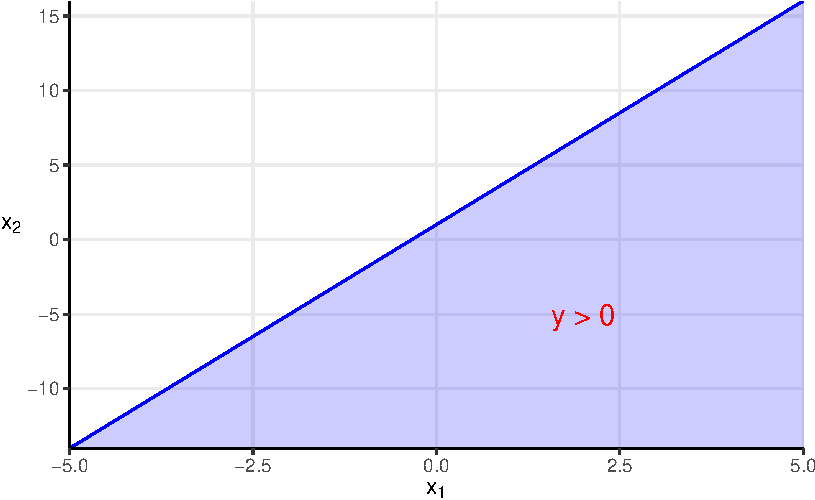
\includegraphics{lista-5_files/figure-pdf/fig-q1a-1.pdf}

}

\caption{\label{fig-q1a}Hiperplano \(1 + 3X_1 - X_2 = 0\)}

\end{figure}%

~

\subsubsection{Item b)}\label{item-b}

On the same plot, sketch the hyperplane \(-2 + X_1 + 2X_2 = 0\).
Indicate the set of points for which \(-2 + X_1 + 2X_2 > 0\), as well as
the set of points for which \(-2 + X_1 + 2X_2 < 0\).

\begin{center}\rule{0.5\linewidth}{0.5pt}\end{center}

~

A Figura~\ref{fig-q1b} mostra o hiperplano indicado da mesma forma que
no item anterior.

~

\begin{figure}[H]

\centering{

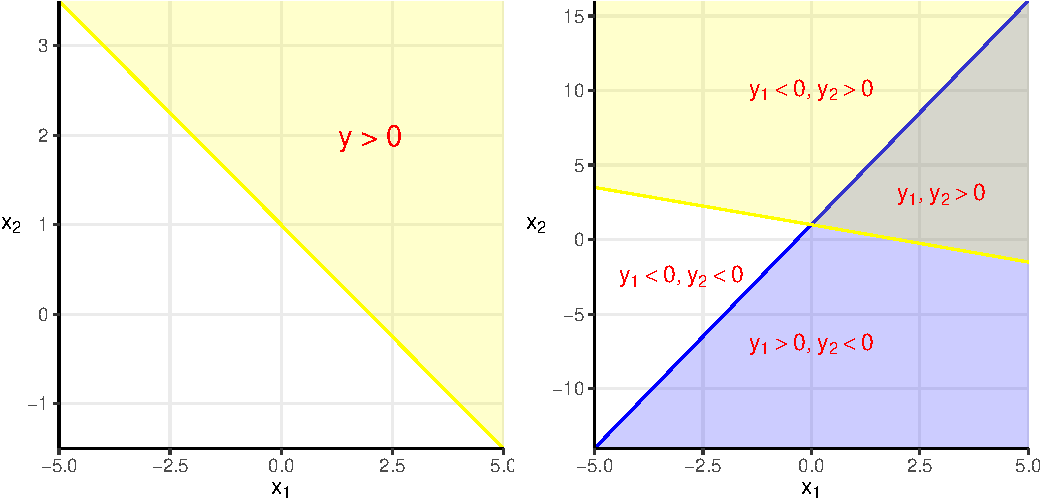
\includegraphics{lista-5_files/figure-pdf/fig-q1b-1.pdf}

}

\caption{\label{fig-q1b}Hiperplano \(-2 + X_1 + 2X_2 = 0\) e interseções
entre os planos}

\end{figure}%

~

\subsection{Questão 2}\label{questuxe3o-2}

We have seen that in \(p = 2\) dimensions, a linear decision boundary
takes the form \(\beta_0 +\beta_1X_1 +\beta_2X_2 = 0\). We now
investigate a non-linear decision boundary.

\subsubsection{Item a)}\label{item-a-1}

Sketch the curve \((1 + X_1)^2 + (2 − X_2)^2 = 4\)

\begin{center}\rule{0.5\linewidth}{0.5pt}\end{center}

A Figura~\ref{fig-q2a} mostra a elipse definida pela equação
\((1 + X_1)^2 + (2 − X_2)^2 = 4\).

\begin{Shaded}
\begin{Highlighting}[]
\NormalTok{x1 }\OtherTok{\textless{}{-}} \FunctionTok{seq}\NormalTok{(}\SpecialCharTok{{-}}\DecValTok{4}\NormalTok{, }\DecValTok{2}\NormalTok{, }\AttributeTok{length.out =} \DecValTok{100}\NormalTok{)}
\NormalTok{x2 }\OtherTok{\textless{}{-}} \FunctionTok{seq}\NormalTok{(}\SpecialCharTok{{-}}\DecValTok{2}\NormalTok{, }\DecValTok{6}\NormalTok{, }\AttributeTok{length.out =} \DecValTok{100}\NormalTok{)}

\NormalTok{grid }\OtherTok{\textless{}{-}} \FunctionTok{expand.grid}\NormalTok{(}\AttributeTok{X1 =}\NormalTok{ x1, }\AttributeTok{X2 =}\NormalTok{ x2)}

\NormalTok{grid}\SpecialCharTok{$}\NormalTok{Z }\OtherTok{\textless{}{-}}\NormalTok{ (}\DecValTok{1} \SpecialCharTok{+}\NormalTok{ grid}\SpecialCharTok{$}\NormalTok{X1)}\SpecialCharTok{\^{}}\DecValTok{2} \SpecialCharTok{+}\NormalTok{ (}\DecValTok{2} \SpecialCharTok{{-}}\NormalTok{ grid}\SpecialCharTok{$}\NormalTok{X2)}\SpecialCharTok{\^{}}\DecValTok{2}

\FunctionTok{ggplot}\NormalTok{(grid, }\FunctionTok{aes}\NormalTok{(}\AttributeTok{x =}\NormalTok{ X1, }\AttributeTok{y =}\NormalTok{ X2, }\AttributeTok{z =}\NormalTok{ Z)) }\SpecialCharTok{+}
  \FunctionTok{geom\_contour}\NormalTok{(}\FunctionTok{aes}\NormalTok{(}\AttributeTok{z =}\NormalTok{ Z), }\AttributeTok{breaks =} \DecValTok{4}\NormalTok{, }\AttributeTok{color =} \StringTok{"black"}\NormalTok{, }\AttributeTok{linewidth =} \DecValTok{1}\NormalTok{) }\SpecialCharTok{+}
  \FunctionTok{labs}\NormalTok{(}
       \AttributeTok{x =} \StringTok{"X1"}\NormalTok{, }\AttributeTok{y =} \StringTok{"X2"}\NormalTok{) }\SpecialCharTok{+}
  \FunctionTok{expand\_limits}\NormalTok{(}\AttributeTok{x =} \FunctionTok{c}\NormalTok{(}\SpecialCharTok{{-}}\DecValTok{4}\NormalTok{, }\DecValTok{2}\NormalTok{), }\AttributeTok{y =} \FunctionTok{c}\NormalTok{(}\SpecialCharTok{{-}}\DecValTok{2}\NormalTok{, }\DecValTok{6}\NormalTok{)) }\SpecialCharTok{+}
  \FunctionTok{theme\_minimal}\NormalTok{()}
\end{Highlighting}
\end{Shaded}

\begin{figure}[H]

\centering{

\captionsetup{labelsep=none}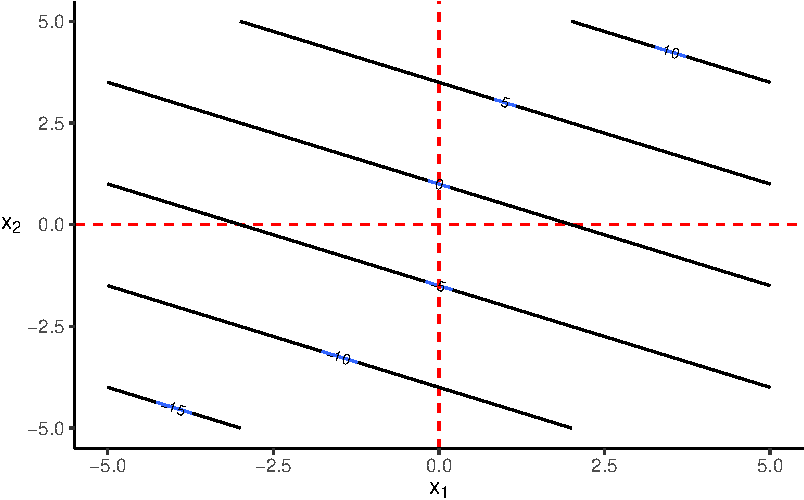
\includegraphics{lista-5_files/figure-pdf/fig-q2a-1.pdf}

}

\caption{\label{fig-q2a}}

\end{figure}%

~

\subsubsection{Item b)}\label{item-b-1}

On your sketch, indicate the set of points for which
\((1 + X_1)^2 + (2 − X_2)^2 > 4\), as well as the set of points for
which \((1 + X_1)^2 + (2 − X_2)^2 \leq 4\).

\begin{center}\rule{0.5\linewidth}{0.5pt}\end{center}

\begin{Shaded}
\begin{Highlighting}[]
\FunctionTok{ggplot}\NormalTok{(}\FunctionTok{subset}\NormalTok{(grid, Z }\SpecialCharTok{\textgreater{}} \DecValTok{4}\NormalTok{), }\FunctionTok{aes}\NormalTok{(}\AttributeTok{x =}\NormalTok{ X1, }\AttributeTok{y =}\NormalTok{ X2)) }\SpecialCharTok{+}
  \FunctionTok{geom\_point}\NormalTok{(}\AttributeTok{color =} \StringTok{"red"}\NormalTok{, }\AttributeTok{alpha =} \FloatTok{0.2}\NormalTok{) }\SpecialCharTok{+}
  \FunctionTok{geom\_point}\NormalTok{(}\AttributeTok{data =} \FunctionTok{subset}\NormalTok{(grid, Z }\SpecialCharTok{\textless{}=} \DecValTok{4}\NormalTok{), }\FunctionTok{aes}\NormalTok{(}\AttributeTok{x =}\NormalTok{ X1, }\AttributeTok{y =}\NormalTok{ X2), }\AttributeTok{color =} \StringTok{"blue"}\NormalTok{, }\AttributeTok{alpha =} \FloatTok{0.2}\NormalTok{)}\SpecialCharTok{+}
  \FunctionTok{labs}\NormalTok{(}
       \AttributeTok{x =} \StringTok{"X1"}\NormalTok{, }\AttributeTok{y =} \StringTok{"X2"}\NormalTok{) }\SpecialCharTok{+}
  \FunctionTok{theme\_minimal}\NormalTok{()}
\end{Highlighting}
\end{Shaded}

\begin{figure}[H]

\centering{

\captionsetup{labelsep=none}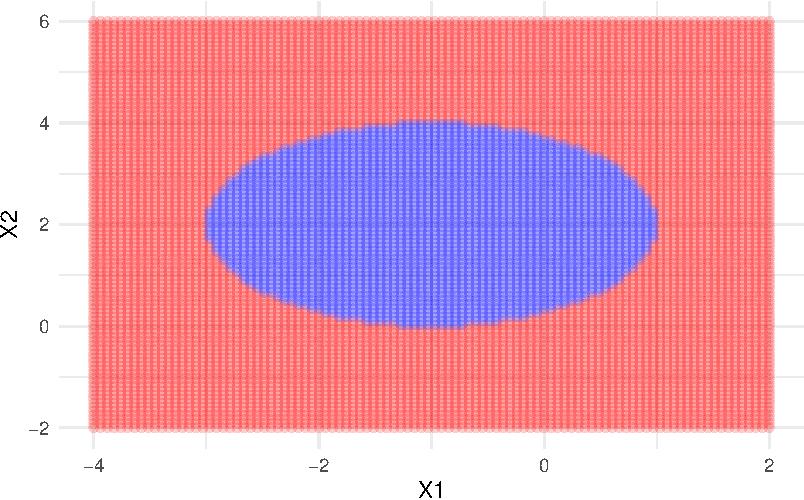
\includegraphics{lista-5_files/figure-pdf/fig-q2b-1.pdf}

}

\caption{\label{fig-q2b}}

\end{figure}%

~

\subsubsection{Item c)}\label{item-c}

Suppose that a classifier assigns an observation to the blue class if
\((1 + X_1)^2 + (2 − X_2)^2 > 4\), and to the red class otherwise. To
what class is the observation (0, 0) classified? (−1, 1)? (2, 2)? (3,
8)?

\begin{center}\rule{0.5\linewidth}{0.5pt}\end{center}

~

Em ordem, teríamos as classificações: azul, vermelho, azul, azul.

\begin{Shaded}
\begin{Highlighting}[]
\NormalTok{theta }\OtherTok{\textless{}{-}} \FunctionTok{seq}\NormalTok{(}\DecValTok{0}\NormalTok{, }\DecValTok{2}\SpecialCharTok{*}\NormalTok{pi, }\AttributeTok{length.out =} \DecValTok{100}\NormalTok{)}

\NormalTok{pontos }\OtherTok{\textless{}{-}} \FunctionTok{tibble}\NormalTok{(}
  \AttributeTok{x =} \FunctionTok{c}\NormalTok{(}\DecValTok{0}\NormalTok{, }\SpecialCharTok{{-}}\DecValTok{1}\NormalTok{, }\DecValTok{2}\NormalTok{, }\DecValTok{3}\NormalTok{),}
  \AttributeTok{y =} \FunctionTok{c}\NormalTok{(}\DecValTok{0}\NormalTok{, }\DecValTok{1}\NormalTok{, }\DecValTok{2}\NormalTok{, }\DecValTok{8}\NormalTok{),}
  \AttributeTok{z =}\NormalTok{ (}\DecValTok{1}\SpecialCharTok{+}\NormalTok{x)}\SpecialCharTok{\^{}}\DecValTok{2} \SpecialCharTok{+}\NormalTok{ (}\DecValTok{2}\SpecialCharTok{{-}}\NormalTok{y)}\SpecialCharTok{\^{}}\DecValTok{2}\NormalTok{, }
  \AttributeTok{cor =}\NormalTok{ z }\SpecialCharTok{\textgreater{}} \DecValTok{4}
\NormalTok{)}

\FunctionTok{ggplot}\NormalTok{(grid, }\FunctionTok{aes}\NormalTok{(}\AttributeTok{x =}\NormalTok{ X1, }\AttributeTok{y =}\NormalTok{ X2, }\AttributeTok{z =}\NormalTok{ Z)) }\SpecialCharTok{+}
  \FunctionTok{geom\_contour}\NormalTok{(}\FunctionTok{aes}\NormalTok{(}\AttributeTok{z =}\NormalTok{ Z), }\AttributeTok{breaks =} \DecValTok{4}\NormalTok{, }\AttributeTok{color =} \StringTok{"black"}\NormalTok{, }\AttributeTok{linewidth =} \DecValTok{1}\NormalTok{) }\SpecialCharTok{+}
  \FunctionTok{geom\_point}\NormalTok{(}\AttributeTok{data =}\NormalTok{ pontos, }\FunctionTok{aes}\NormalTok{(}\AttributeTok{x =}\NormalTok{ x, }\AttributeTok{y =}\NormalTok{ y, }\AttributeTok{z =}\NormalTok{ z, }\AttributeTok{color =}\NormalTok{ cor), }\AttributeTok{size =} \DecValTok{3}\NormalTok{) }\SpecialCharTok{+}
  \FunctionTok{labs}\NormalTok{(}\AttributeTok{color =} \StringTok{"Z \textgreater{} 4"}\NormalTok{,}
       \AttributeTok{x =} \StringTok{"X1"}\NormalTok{, }\AttributeTok{y =} \StringTok{"X2"}\NormalTok{) }\SpecialCharTok{+}
  \FunctionTok{expand\_limits}\NormalTok{(}\AttributeTok{x =} \FunctionTok{c}\NormalTok{(}\SpecialCharTok{{-}}\DecValTok{4}\NormalTok{, }\DecValTok{2}\NormalTok{), }\AttributeTok{y =} \FunctionTok{c}\NormalTok{(}\SpecialCharTok{{-}}\DecValTok{2}\NormalTok{, }\DecValTok{6}\NormalTok{)) }\SpecialCharTok{+}
  \FunctionTok{theme\_minimal}\NormalTok{()}
\end{Highlighting}
\end{Shaded}

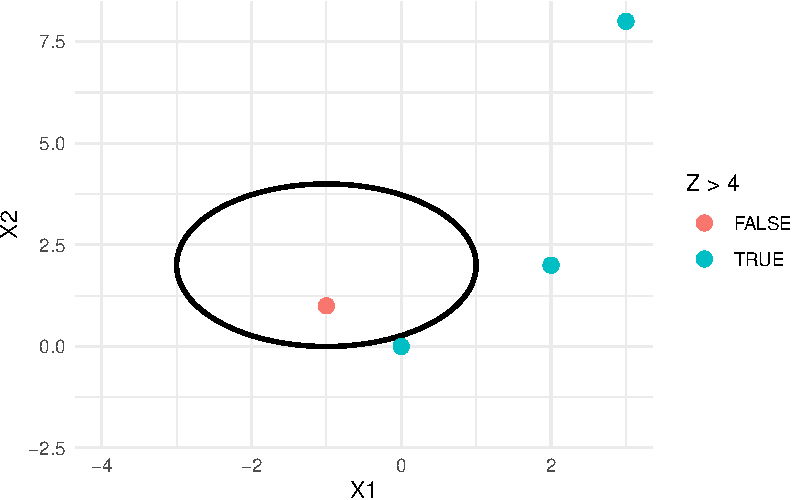
\includegraphics{lista-5_files/figure-pdf/unnamed-chunk-6-1.pdf}

~

~

\subsubsection{Item d)}\label{item-d}

Argue that while the decision boundary in (c) is not linear in terms of
\(X_1\) and \(X_2\), it is linear in terms of \(X_1\), \(X^2_1\),
\(X_2\), and \(X^2_2\).

\begin{center}\rule{0.5\linewidth}{0.5pt}\end{center}

De fato, se expandirmos a equação, temos

\[
(1 + X_1)^2 + (2 - X_2)^2 = 4 \\ 
1 + 2X_1 + X^2_1 + 4 - 4X_2 + X^2_2 = 4 \\
X^2_1 + X^2_2 +2X_1 - 4X_2 +1 = 0, 
\] que é linear com respeito a \(X_1\), \(X^2_1\), \(X_2\), e \(X^2_2\).

~

\subsection{Questão 3}\label{questuxe3o-3}

Here we explore the maximal margin classifier on a toy data set.

\subsubsection{Item a)}\label{item-a-2}

We are given n = 7 observations in p = 2 dimensions. For each
observation, there is an associated class label. Sketch the
observations.

\begin{center}\rule{0.5\linewidth}{0.5pt}\end{center}

~

Criando o banco de dados do exercicio e fazendo um gráfico dele.

\begin{Shaded}
\begin{Highlighting}[]
\NormalTok{df }\OtherTok{\textless{}{-}} \FunctionTok{data.frame}\NormalTok{(}
  \AttributeTok{Obs =} \DecValTok{1}\SpecialCharTok{:}\DecValTok{7}\NormalTok{,}
  \AttributeTok{X1 =} \FunctionTok{c}\NormalTok{(}\DecValTok{3}\NormalTok{, }\DecValTok{2}\NormalTok{, }\DecValTok{4}\NormalTok{, }\DecValTok{1}\NormalTok{, }\DecValTok{2}\NormalTok{, }\DecValTok{4}\NormalTok{, }\DecValTok{4}\NormalTok{),}
  \AttributeTok{X2 =} \FunctionTok{c}\NormalTok{(}\DecValTok{4}\NormalTok{, }\DecValTok{2}\NormalTok{, }\DecValTok{4}\NormalTok{, }\DecValTok{4}\NormalTok{, }\DecValTok{1}\NormalTok{, }\DecValTok{3}\NormalTok{, }\DecValTok{1}\NormalTok{),}
  \AttributeTok{Y =} \FunctionTok{c}\NormalTok{(}\StringTok{"Red"}\NormalTok{, }\StringTok{"Red"}\NormalTok{, }\StringTok{"Red"}\NormalTok{, }\StringTok{"Red"}\NormalTok{, }\StringTok{"Blue"}\NormalTok{, }\StringTok{"Blue"}\NormalTok{, }\StringTok{"Blue"}\NormalTok{)}
\NormalTok{)}
\FunctionTok{ggplot}\NormalTok{(df, }\FunctionTok{aes}\NormalTok{(}\AttributeTok{x =}\NormalTok{ X1, }\AttributeTok{y =}\NormalTok{ X2, }\AttributeTok{color =}\NormalTok{ Y)) }\SpecialCharTok{+}
  \FunctionTok{geom\_point}\NormalTok{(}\AttributeTok{size =} \DecValTok{3}\NormalTok{) }\SpecialCharTok{+}
  \FunctionTok{scale\_color\_manual}\NormalTok{(}\AttributeTok{values =} \FunctionTok{c}\NormalTok{(}\StringTok{"Red"} \OtherTok{=} \StringTok{"red"}\NormalTok{, }\StringTok{"Blue"} \OtherTok{=} \StringTok{"blue"}\NormalTok{)) }\SpecialCharTok{+}
  \FunctionTok{labs}\NormalTok{(}\AttributeTok{x =} \StringTok{"X1"}\NormalTok{, }\AttributeTok{y =} \StringTok{"X2"}\NormalTok{, }\AttributeTok{title =} \StringTok{"Plot of Observations"}\NormalTok{) }\SpecialCharTok{+}
  \FunctionTok{theme\_minimal}\NormalTok{()}
\end{Highlighting}
\end{Shaded}

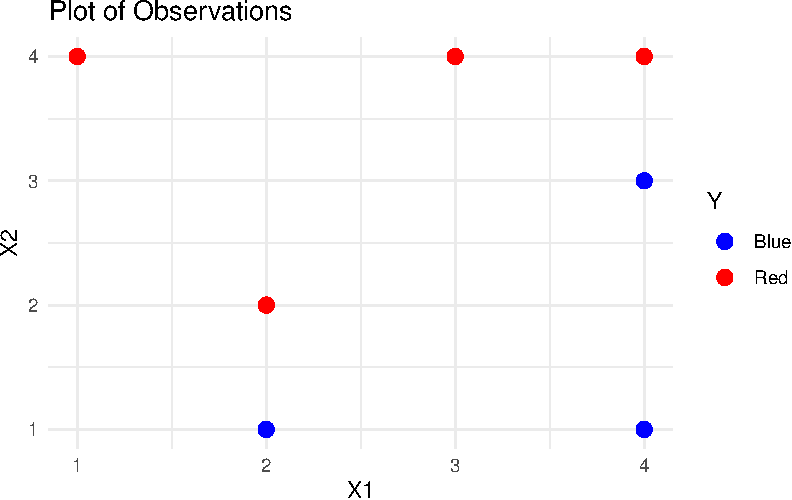
\includegraphics{lista-5_files/figure-pdf/unnamed-chunk-7-1.pdf}

~

\subsubsection{Item b)}\label{item-b-2}

Sketch the optimal separating hyperplane, and provide the equation for
this hyperplane (of the form (9.1)).

~

Os pontos (x1,x2)=(2,2) e (4,3) parecem ser 2 bons pontos para se fazer
hiperplano ótimo de separação.

\begin{Shaded}
\begin{Highlighting}[]
\CommentTok{\# Calcular os coeficientes}
\NormalTok{ponto1 }\OtherTok{\textless{}{-}} \FunctionTok{c}\NormalTok{(}\DecValTok{2}\NormalTok{, }\DecValTok{2}\NormalTok{)}
\NormalTok{ponto2 }\OtherTok{\textless{}{-}} \FunctionTok{c}\NormalTok{(}\DecValTok{4}\NormalTok{, }\DecValTok{3}\NormalTok{)}

\CommentTok{\# Inclinação da reta}
\NormalTok{m }\OtherTok{\textless{}{-}}\NormalTok{ (ponto2[}\DecValTok{2}\NormalTok{] }\SpecialCharTok{{-}}\NormalTok{ ponto1[}\DecValTok{2}\NormalTok{]) }\SpecialCharTok{/}\NormalTok{ (ponto2[}\DecValTok{1}\NormalTok{] }\SpecialCharTok{{-}}\NormalTok{ ponto1[}\DecValTok{1}\NormalTok{])}

\CommentTok{\# intercept}
\NormalTok{b }\OtherTok{\textless{}{-}}\NormalTok{ ponto1[}\DecValTok{2}\NormalTok{] }\SpecialCharTok{{-}}\NormalTok{ m }\SpecialCharTok{*}\NormalTok{ ponto1[}\DecValTok{1}\NormalTok{]}

\CommentTok{\# Equação da linha: X2 = m * X1 + b}
\CommentTok{\# Converter para a forma: beta\_1 * X1 + beta\_2 * X2 + beta\_0 = 0}
\NormalTok{beta1 }\OtherTok{\textless{}{-}} \SpecialCharTok{{-}}\NormalTok{m}
\NormalTok{beta2 }\OtherTok{\textless{}{-}} \DecValTok{1}
\NormalTok{beta0 }\OtherTok{\textless{}{-}} \SpecialCharTok{{-}}\NormalTok{b}

\CommentTok{\# Plotar com o hiperplano}
\FunctionTok{ggplot}\NormalTok{(df, }\FunctionTok{aes}\NormalTok{(}\AttributeTok{x =}\NormalTok{ X1, }\AttributeTok{y =}\NormalTok{ X2, }\AttributeTok{color =}\NormalTok{ Y)) }\SpecialCharTok{+}
  \FunctionTok{geom\_point}\NormalTok{(}\AttributeTok{size =} \DecValTok{4}\NormalTok{) }\SpecialCharTok{+}
  \FunctionTok{geom\_abline}\NormalTok{(}\AttributeTok{intercept =}\NormalTok{ b, }\AttributeTok{slope =}\NormalTok{ m, }\AttributeTok{color =} \StringTok{"black"}\NormalTok{) }\SpecialCharTok{+}
  \FunctionTok{labs}\NormalTok{(}\AttributeTok{title =} \StringTok{"Hiperplano de Separação Ótimo"}\NormalTok{) }\SpecialCharTok{+}
  \FunctionTok{theme\_minimal}\NormalTok{()}
\end{Highlighting}
\end{Shaded}

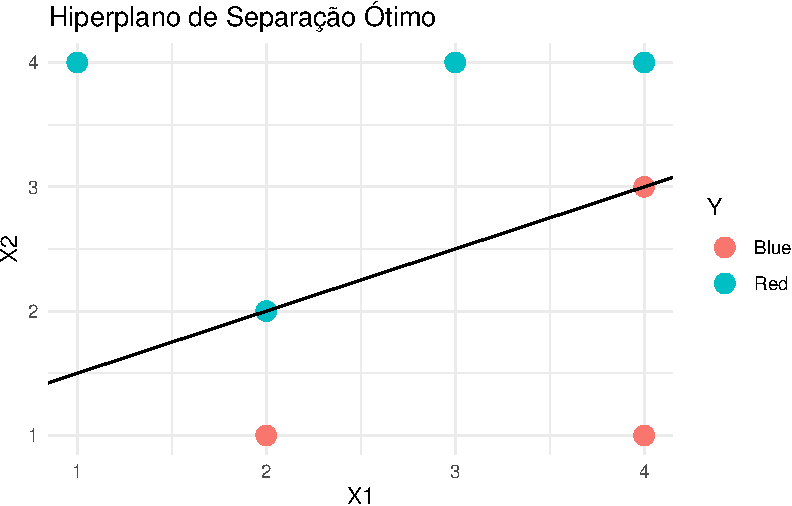
\includegraphics{lista-5_files/figure-pdf/unnamed-chunk-8-1.pdf}

\begin{Shaded}
\begin{Highlighting}[]
\FunctionTok{cat}\NormalTok{(}\StringTok{"Equação do hiperplano: "}\NormalTok{)}
\end{Highlighting}
\end{Shaded}

\begin{verbatim}
Equação do hiperplano: 
\end{verbatim}

\begin{Shaded}
\begin{Highlighting}[]
\FunctionTok{cat}\NormalTok{(}\FunctionTok{paste0}\NormalTok{(beta0, }\StringTok{" + "}\NormalTok{, beta1, }\StringTok{" * X1 + "}\NormalTok{, beta2, }\StringTok{" * X2 = 0"}\NormalTok{))}
\end{Highlighting}
\end{Shaded}

\begin{verbatim}
-1 + -0.5 * X1 + 1 * X2 = 0
\end{verbatim}

~

\subsubsection{Item c)}\label{item-c-1}

Describe the classification rule for the maximal margin classifier. It
should be something along the lines of ``Classify to Red if
\(\beta_0 + \beta_1X_1 + \beta_2X_2 > 0\), and classify to Blue
otherwise.'' Provide the values for \(\beta_0\), \(\beta_1\), and
\(\beta_2\).

\begin{center}\rule{0.5\linewidth}{0.5pt}\end{center}

\begin{Shaded}
\begin{Highlighting}[]
\FunctionTok{cat}\NormalTok{(}\StringTok{"Se "}\NormalTok{)}
\end{Highlighting}
\end{Shaded}

\begin{verbatim}
Se 
\end{verbatim}

\begin{Shaded}
\begin{Highlighting}[]
\FunctionTok{cat}\NormalTok{(}\FunctionTok{paste0}\NormalTok{(beta0, }\StringTok{" + "}\NormalTok{, beta1, }\StringTok{" * X1 + "}\NormalTok{, beta2, }\StringTok{" * X2 \textgreater{} 0"}\NormalTok{),}\StringTok{"classifique como vermelho e azul caso contrario"}\NormalTok{)}
\end{Highlighting}
\end{Shaded}

\begin{verbatim}
-1 + -0.5 * X1 + 1 * X2 > 0 classifique como vermelho e azul caso contrario
\end{verbatim}

~

\subsubsection{Item d)}\label{item-d-1}

On your sketch, indicate the margin for the maximal margin hyperplane.

\begin{center}\rule{0.5\linewidth}{0.5pt}\end{center}

\begin{Shaded}
\begin{Highlighting}[]
\CommentTok{\# Calcular a margem}
\NormalTok{margem }\OtherTok{\textless{}{-}} \DecValTok{1} \SpecialCharTok{/} \FunctionTok{sqrt}\NormalTok{(beta1}\SpecialCharTok{\^{}}\DecValTok{2} \SpecialCharTok{+}\NormalTok{ beta2}\SpecialCharTok{\^{}}\DecValTok{2}\NormalTok{)}

\CommentTok{\# Adicionar linhas de margem}
\FunctionTok{ggplot}\NormalTok{(df, }\FunctionTok{aes}\NormalTok{(}\AttributeTok{x =}\NormalTok{ X1, }\AttributeTok{y =}\NormalTok{ X2, }\AttributeTok{color =}\NormalTok{ Y)) }\SpecialCharTok{+}
  \FunctionTok{geom\_point}\NormalTok{(}\AttributeTok{size =} \DecValTok{4}\NormalTok{) }\SpecialCharTok{+}
  \FunctionTok{geom\_abline}\NormalTok{(}\AttributeTok{intercept =}\NormalTok{ b, }\AttributeTok{slope =}\NormalTok{ m, }\AttributeTok{color =} \StringTok{"black"}\NormalTok{) }\SpecialCharTok{+}
  \FunctionTok{labs}\NormalTok{(}\AttributeTok{title =} \StringTok{"Hiperplano de Separação Ótimo"}\NormalTok{) }\SpecialCharTok{+}
  \FunctionTok{theme\_minimal}\NormalTok{()}\SpecialCharTok{+}
  \FunctionTok{geom\_abline}\NormalTok{(}\AttributeTok{intercept =}\NormalTok{ (b }\SpecialCharTok{+}\NormalTok{ margem }\SpecialCharTok{/}\NormalTok{ beta2), }\AttributeTok{slope =}\NormalTok{ m, }\AttributeTok{linetype =} \StringTok{"dotted"}\NormalTok{) }\SpecialCharTok{+}
  \FunctionTok{geom\_abline}\NormalTok{(}\AttributeTok{intercept =}\NormalTok{ (b }\SpecialCharTok{{-}}\NormalTok{ margem }\SpecialCharTok{/}\NormalTok{ beta2), }\AttributeTok{slope =}\NormalTok{ m, }\AttributeTok{linetype =} \StringTok{"dotted"}\NormalTok{)}
\end{Highlighting}
\end{Shaded}

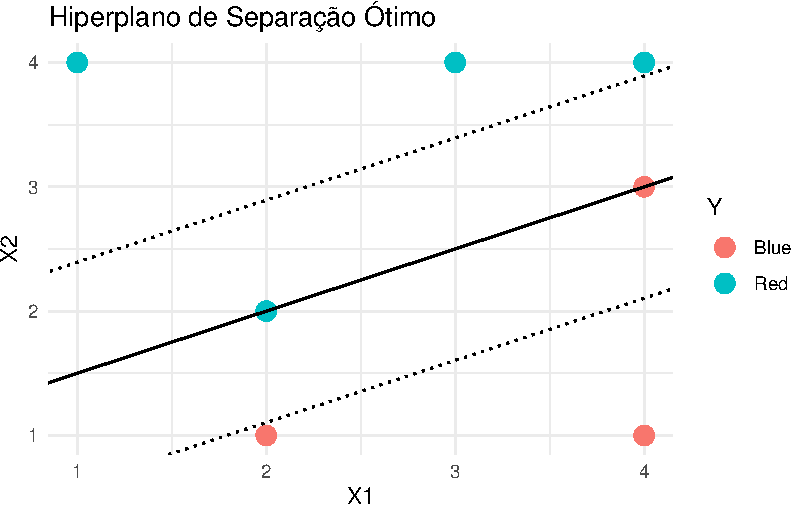
\includegraphics{lista-5_files/figure-pdf/unnamed-chunk-11-1.pdf}

~

\subsubsection{Item e)}\label{item-e}

Indicate the support vectors for the maximal margin classifier.

\begin{center}\rule{0.5\linewidth}{0.5pt}\end{center}

~

Os pontos (x1,x2)=(2,2) e (4,3) foram usados como vetores de suporte.

~

\subsubsection{Item f)}\label{item-f}

Argue that a slight movement of the seventh observation would not affect
the maximal margin hyperplane.

\begin{center}\rule{0.5\linewidth}{0.5pt}\end{center}

~

Um movimento pequeno no ponto (4,1) não afetaria a margem máxima do
hiperplano visto que está distante da mesma e não é um dos vetores de
suporte. ~

\subsubsection{Item g)}\label{item-g}

Sketch a hyperplane that is not the optimal separating hyperplane, and
provide the equation for this hyperplane.

\begin{center}\rule{0.5\linewidth}{0.5pt}\end{center}

~

\begin{Shaded}
\begin{Highlighting}[]
\CommentTok{\# Hiperplano não ótimo}
\FunctionTok{ggplot}\NormalTok{(df, }\FunctionTok{aes}\NormalTok{(}\AttributeTok{x =}\NormalTok{ X1, }\AttributeTok{y =}\NormalTok{ X2, }\AttributeTok{color =}\NormalTok{ Y)) }\SpecialCharTok{+}
  \FunctionTok{geom\_point}\NormalTok{(}\AttributeTok{size =} \DecValTok{4}\NormalTok{) }\SpecialCharTok{+}
  \FunctionTok{geom\_abline}\NormalTok{(}\AttributeTok{intercept =} \DecValTok{5}\NormalTok{, }\AttributeTok{slope =} \SpecialCharTok{{-}}\DecValTok{1}\NormalTok{, }\AttributeTok{color =} \StringTok{"red"}\NormalTok{, }\AttributeTok{linetype =} \StringTok{"dashed"}\NormalTok{) }\SpecialCharTok{+}
  \FunctionTok{labs}\NormalTok{(}\AttributeTok{title =} \StringTok{"Hiperplano de Separação Não Ótimo"}\NormalTok{) }\SpecialCharTok{+}
  \FunctionTok{theme\_minimal}\NormalTok{()}
\end{Highlighting}
\end{Shaded}

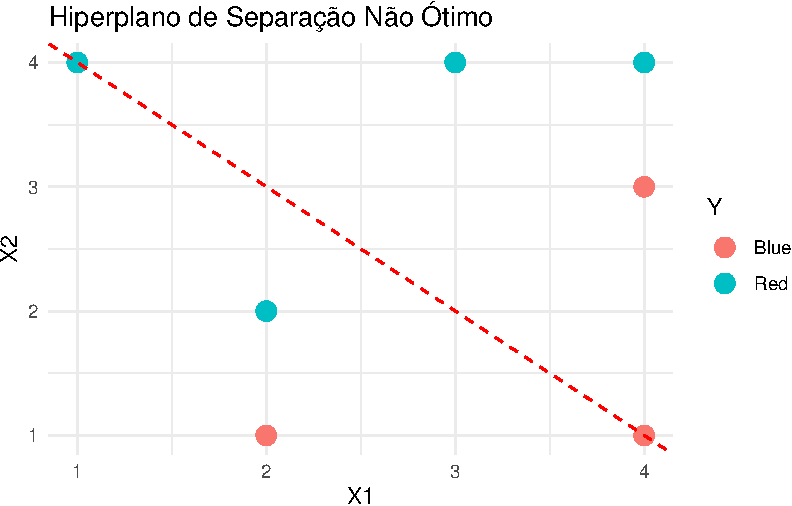
\includegraphics{lista-5_files/figure-pdf/unnamed-chunk-12-1.pdf}

~

\subsubsection{Item h)}\label{item-h}

Draw an additional observation on the plot so that the two classes are
no longer separable by a hyperplane.

\begin{center}\rule{0.5\linewidth}{0.5pt}\end{center}

~

\begin{Shaded}
\begin{Highlighting}[]
\CommentTok{\# Adicionar nova observação}
\NormalTok{df2 }\OtherTok{\textless{}{-}} \FunctionTok{rbind}\NormalTok{(df, }\FunctionTok{data.frame}\NormalTok{(}\AttributeTok{X1 =} \DecValTok{3}\NormalTok{, }\AttributeTok{X2 =} \DecValTok{3}\NormalTok{, }\AttributeTok{Y =} \FunctionTok{as.factor}\NormalTok{(}\StringTok{\textquotesingle{}Blue\textquotesingle{}}\NormalTok{),}\AttributeTok{Obs=}\DecValTok{8}\NormalTok{))}

\CommentTok{\# Plotar}
\FunctionTok{ggplot}\NormalTok{(df2, }\FunctionTok{aes}\NormalTok{(}\AttributeTok{x =}\NormalTok{ X1, }\AttributeTok{y =}\NormalTok{ X2, }\AttributeTok{color =}\NormalTok{ Y)) }\SpecialCharTok{+}
  \FunctionTok{geom\_point}\NormalTok{(}\AttributeTok{size =} \DecValTok{4}\NormalTok{) }\SpecialCharTok{+}
  \FunctionTok{labs}\NormalTok{(}\AttributeTok{title =} \StringTok{"Classes não separaveis com uma nova observação"}\NormalTok{) }\SpecialCharTok{+}
  \FunctionTok{theme\_minimal}\NormalTok{()}
\end{Highlighting}
\end{Shaded}

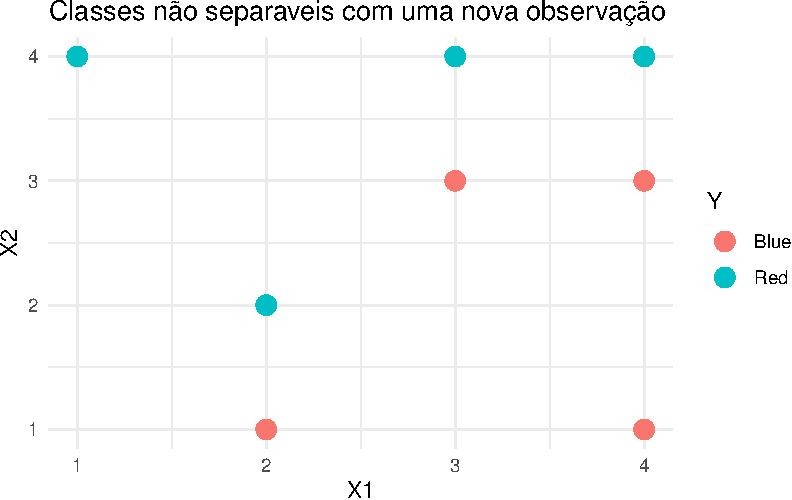
\includegraphics{lista-5_files/figure-pdf/unnamed-chunk-13-1.pdf}

~

\subsection{Questão 4}\label{questuxe3o-4}

Generate a simulated two-class data set with 100 observations and two
features in which there is a visible but non-linear separation between
the two classes. Show that in this setting, a support vector machine
with a polynomial kernel (with degree greater than 1) or a radial kernel
will outperform a support vector classifier on the training data. Which
technique performs best on the test data? Make plots and report training
and test error rates in order to back up your assertions.

\begin{center}\rule{0.5\linewidth}{0.5pt}\end{center}

~

Os dados são gerados a seguir, seguidos de um gráfico mostrando a
separação entre as classes.

\begin{Shaded}
\begin{Highlighting}[]
\FunctionTok{set.seed}\NormalTok{ (}\DecValTok{1}\NormalTok{)}
\NormalTok{x }\OtherTok{\textless{}{-}} \FunctionTok{matrix}\NormalTok{(}\FunctionTok{rnorm}\NormalTok{ (}\DecValTok{100} \SpecialCharTok{*} \DecValTok{2}\NormalTok{), }\AttributeTok{ncol =} \DecValTok{2}\NormalTok{)}
\NormalTok{x[}\DecValTok{1}\SpecialCharTok{:}\DecValTok{25}\NormalTok{, ] }\OtherTok{\textless{}{-}}\NormalTok{ x[}\DecValTok{1}\SpecialCharTok{:}\DecValTok{25}\NormalTok{, ] }\SpecialCharTok{+} \DecValTok{2}
\NormalTok{x[}\DecValTok{76}\SpecialCharTok{:}\DecValTok{100}\NormalTok{, ] }\OtherTok{\textless{}{-}}\NormalTok{ x[}\DecValTok{76}\SpecialCharTok{:}\DecValTok{100}\NormalTok{, ] }\SpecialCharTok{{-}} \DecValTok{2}
\NormalTok{y }\OtherTok{\textless{}{-}} \FunctionTok{c}\NormalTok{(}\FunctionTok{rep}\NormalTok{(}\DecValTok{1}\NormalTok{, }\DecValTok{25}\NormalTok{), }\FunctionTok{rep}\NormalTok{(}\DecValTok{2}\NormalTok{, }\DecValTok{50}\NormalTok{), }\FunctionTok{rep}\NormalTok{(}\DecValTok{1}\NormalTok{, }\DecValTok{25}\NormalTok{))}
\NormalTok{dat }\OtherTok{\textless{}{-}} \FunctionTok{data.frame}\NormalTok{(}\AttributeTok{x =}\NormalTok{ x, }\AttributeTok{y =} \FunctionTok{as.factor}\NormalTok{(y))}

\FunctionTok{plot}\NormalTok{(x, }\AttributeTok{col =}\NormalTok{ y)}
\end{Highlighting}
\end{Shaded}

\begin{figure}[H]

\centering{

\captionsetup{labelsep=none}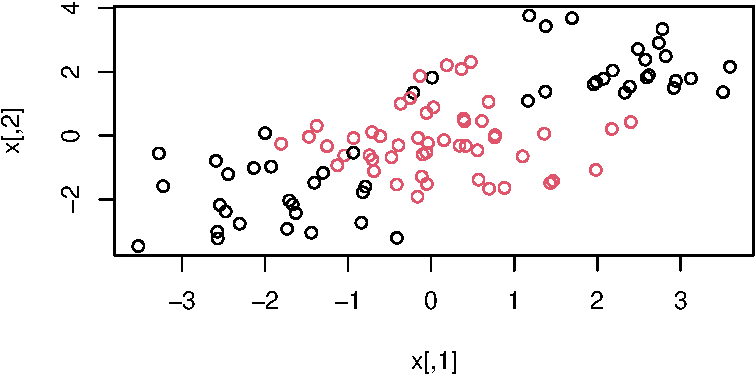
\includegraphics{lista-5_files/figure-pdf/fig-q4-1.pdf}

}

\caption{\label{fig-q4}}

\end{figure}%

~

A seguir são ajustados os modelos SVM com kernel polinomial e radial,
bem como o modelo SVM linear. Os resultados para uma partição de teste
são apresentados na tabela a seguir utilizando custo igual a 1 em todos
os casos, grau de polinômio igual a 2 no caso polinomial e \(\gamma\)
igual a 1 no caso radial.

\begin{Shaded}
\begin{Highlighting}[]
\CommentTok{\# seleciona parte da base como teste = 1}
\FunctionTok{set.seed}\NormalTok{(}\DecValTok{1}\NormalTok{)}
\NormalTok{test }\OtherTok{\textless{}{-}} \FunctionTok{sample}\NormalTok{(}\FunctionTok{c}\NormalTok{(}\DecValTok{1}\NormalTok{, }\DecValTok{0}\NormalTok{), }\DecValTok{100}\NormalTok{, }\AttributeTok{replace =} \ConstantTok{TRUE}\NormalTok{, }\AttributeTok{prob =} \FunctionTok{c}\NormalTok{(}\FloatTok{0.2}\NormalTok{, }\FloatTok{0.8}\NormalTok{))}

\CommentTok{\# classificador linear}
\NormalTok{linearfit }\OtherTok{\textless{}{-}} \FunctionTok{svm}\NormalTok{(y }\SpecialCharTok{\textasciitilde{}}\NormalTok{ ., }\AttributeTok{data =}\NormalTok{ dat[test }\SpecialCharTok{==} \DecValTok{0}\NormalTok{,] , }\AttributeTok{kernel =} \StringTok{"linear"}\NormalTok{,}
              \AttributeTok{cost =} \DecValTok{1}\NormalTok{, }\AttributeTok{scale =} \ConstantTok{FALSE}\NormalTok{)}

\CommentTok{\# classificador polinomial}
\NormalTok{polyfit }\OtherTok{\textless{}{-}} \FunctionTok{svm}\NormalTok{(y }\SpecialCharTok{\textasciitilde{}}\NormalTok{ ., }\AttributeTok{data =}\NormalTok{ dat[test }\SpecialCharTok{==} \DecValTok{0}\NormalTok{,] , }\AttributeTok{kernel =} \StringTok{"polynomial"}\NormalTok{,}
              \AttributeTok{degree =} \DecValTok{2}\NormalTok{, }\AttributeTok{cost =} \DecValTok{1}\NormalTok{, }\AttributeTok{scale =} \ConstantTok{FALSE}\NormalTok{)}

\CommentTok{\# classificador radial}
\NormalTok{radialfit }\OtherTok{\textless{}{-}} \FunctionTok{svm}\NormalTok{(y }\SpecialCharTok{\textasciitilde{}}\NormalTok{ ., }\AttributeTok{data =}\NormalTok{ dat[test }\SpecialCharTok{==} \DecValTok{0}\NormalTok{,] , }\AttributeTok{kernel =} \StringTok{"radial"}\NormalTok{,}
              \AttributeTok{gamma =} \DecValTok{1}\NormalTok{, }\AttributeTok{cost =} \DecValTok{1}\NormalTok{, }\AttributeTok{scale =} \ConstantTok{FALSE}\NormalTok{)}

\CommentTok{\# plots utilizando dados de treinamento}
\FunctionTok{plot}\NormalTok{(linearfit, dat[test }\SpecialCharTok{==} \DecValTok{0}\NormalTok{,])}
\end{Highlighting}
\end{Shaded}

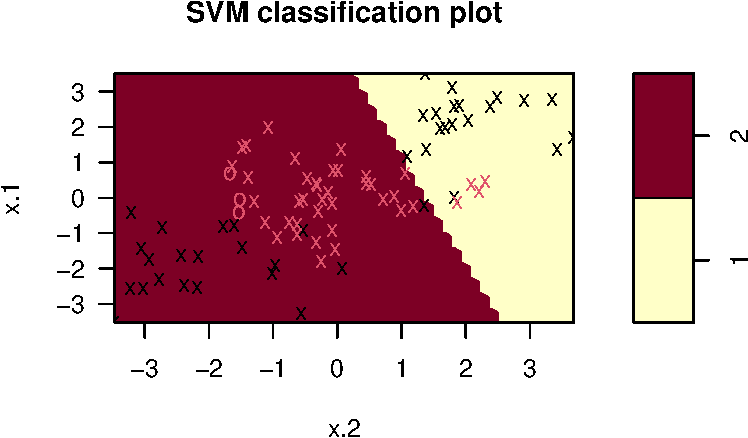
\includegraphics{lista-5_files/figure-pdf/svmfit-1.pdf}

\begin{Shaded}
\begin{Highlighting}[]
\FunctionTok{plot}\NormalTok{(polyfit, dat[test }\SpecialCharTok{==} \DecValTok{0}\NormalTok{,])}
\end{Highlighting}
\end{Shaded}

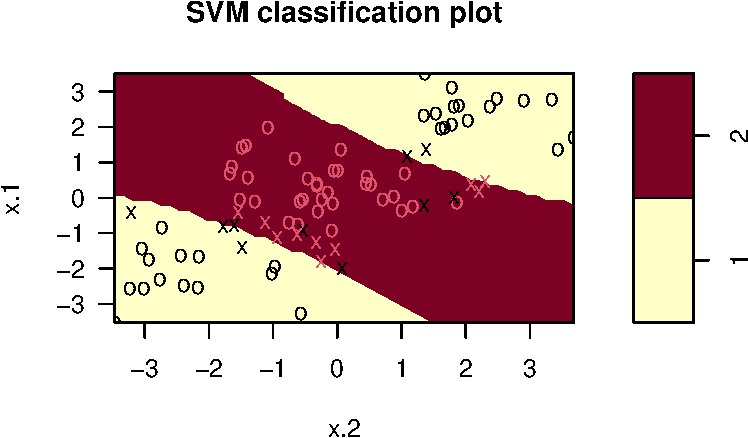
\includegraphics{lista-5_files/figure-pdf/svmfit-2.pdf}

\begin{Shaded}
\begin{Highlighting}[]
\FunctionTok{plot}\NormalTok{(radialfit, dat[test }\SpecialCharTok{==} \DecValTok{0}\NormalTok{,])}
\end{Highlighting}
\end{Shaded}

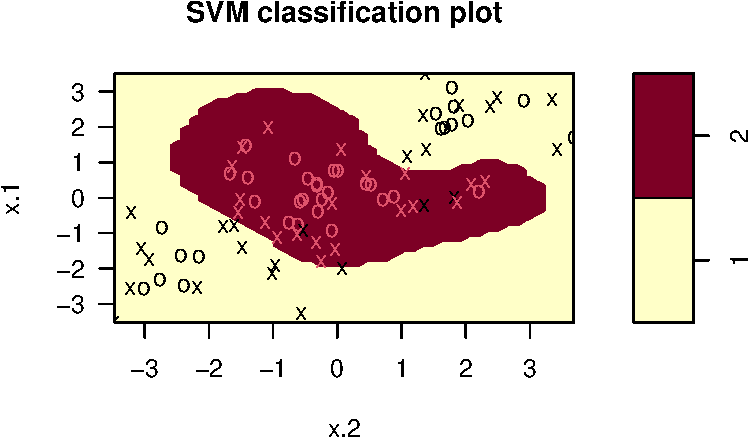
\includegraphics{lista-5_files/figure-pdf/svmfit-3.pdf}

~

Visualmente, o modelo SVM com kernel polinomial parece ser o que melhor
se ajusta aos dados, contando apenas os vetores próximos à fronteira,
como esperado, como vetores de suporte. A tabela a seguir mostra os
resultados para os modelos ajustados com os dados de treinamento.

~

\begin{Shaded}
\begin{Highlighting}[]
\CommentTok{\# table for linear fit}
\NormalTok{tbl\_linear }\OtherTok{\textless{}{-}} \FunctionTok{table}\NormalTok{(}
  \AttributeTok{true =}\NormalTok{ dat[test }\SpecialCharTok{==} \DecValTok{0}\NormalTok{, }\StringTok{"y"}\NormalTok{],}
  \AttributeTok{pred =} \FunctionTok{predict}\NormalTok{(}
\NormalTok{    linearfit , }\AttributeTok{newdata =}\NormalTok{ dat[test }\SpecialCharTok{==} \DecValTok{0}\NormalTok{, ]}
\NormalTok{  )}
\NormalTok{)}

\CommentTok{\# table for poly fit}
\NormalTok{tbl\_poly }\OtherTok{\textless{}{-}} \FunctionTok{table}\NormalTok{(}
  \AttributeTok{true =}\NormalTok{ dat[test }\SpecialCharTok{==} \DecValTok{0}\NormalTok{, }\StringTok{"y"}\NormalTok{],}
  \AttributeTok{pred =} \FunctionTok{predict}\NormalTok{(}
\NormalTok{    polyfit , }\AttributeTok{newdata =}\NormalTok{ dat[test }\SpecialCharTok{==} \DecValTok{0}\NormalTok{, ]}
\NormalTok{  )}
\NormalTok{)}

\CommentTok{\# table for radial fit}
\NormalTok{tbl\_radial }\OtherTok{\textless{}{-}} \FunctionTok{table}\NormalTok{(}
  \AttributeTok{true =}\NormalTok{ dat[test }\SpecialCharTok{==} \DecValTok{0}\NormalTok{, }\StringTok{"y"}\NormalTok{],}
  \AttributeTok{pred =} \FunctionTok{predict}\NormalTok{(}
\NormalTok{    radialfit , }\AttributeTok{newdata =}\NormalTok{ dat[test }\SpecialCharTok{==} \DecValTok{0}\NormalTok{, ]}
\NormalTok{  )}
\NormalTok{)}

\FunctionTok{map}\NormalTok{(}\FunctionTok{list}\NormalTok{(tbl\_linear, tbl\_poly, tbl\_radial), }\ControlFlowTok{function}\NormalTok{(x) \{}
\NormalTok{  x }\SpecialCharTok{\%\textgreater{}\%}
    \FunctionTok{as.data.frame}\NormalTok{() }\SpecialCharTok{\%\textgreater{}\%}
    \FunctionTok{rename}\NormalTok{(}\StringTok{"True"} \OtherTok{=} \StringTok{"true"}\NormalTok{, }\StringTok{"Predicted"} \OtherTok{=} \StringTok{"pred"}\NormalTok{) }\SpecialCharTok{\%\textgreater{}\%}
    \FunctionTok{mutate\_all}\NormalTok{(as.character) }\SpecialCharTok{\%\textgreater{}\%}
    \FunctionTok{mutate}\NormalTok{(}\AttributeTok{True =} \FunctionTok{if\_else}\NormalTok{(True }\SpecialCharTok{==} \StringTok{"1"}\NormalTok{, }\StringTok{"Classe real 1"}\NormalTok{, }\StringTok{"Classe real 2"}\NormalTok{),}
           \AttributeTok{Predicted =} \FunctionTok{if\_else}\NormalTok{(Predicted }\SpecialCharTok{==} \StringTok{"1"}\NormalTok{, }\StringTok{"Classe fit 1"}\NormalTok{, }\StringTok{"Classe fit 2"}\NormalTok{)) }\SpecialCharTok{\%\textgreater{}\%}
    \FunctionTok{pivot\_wider}\NormalTok{(}\AttributeTok{names\_from =} \StringTok{"True"}\NormalTok{, }\AttributeTok{values\_from =} \StringTok{"Freq"}\NormalTok{)}
\NormalTok{\}) }\SpecialCharTok{\%\textgreater{}\%}
  \FunctionTok{bind\_rows}\NormalTok{() }\SpecialCharTok{\%\textgreater{}\%}
  \FunctionTok{mutate}\NormalTok{(}\AttributeTok{Modelo =} \FunctionTok{rep}\NormalTok{(}\FunctionTok{c}\NormalTok{(}\StringTok{"Linear"}\NormalTok{, }\StringTok{"Polinomial"}\NormalTok{, }\StringTok{"Radial"}\NormalTok{), }\AttributeTok{each =} \DecValTok{2}\NormalTok{)) }\SpecialCharTok{\%\textgreater{}\%}
  \FunctionTok{select}\NormalTok{(Modelo, }\FunctionTok{everything}\NormalTok{()) }\SpecialCharTok{\%\textgreater{}\%}
\NormalTok{  knitr}\SpecialCharTok{::}\FunctionTok{kable}\NormalTok{(}\AttributeTok{caption =} \StringTok{"Matriz de confusão para os modelos ajustados com os dados de treinamento"}\NormalTok{)}
\end{Highlighting}
\end{Shaded}

\begin{longtable}[]{@{}llll@{}}
\caption{Matriz de confusão para os modelos ajustados com os dados de
treinamento}\tabularnewline
\toprule\noalign{}
Modelo & Predicted & Classe real 1 & Classe real 2 \\
\midrule\noalign{}
\endfirsthead
\toprule\noalign{}
Modelo & Predicted & Classe real 1 & Classe real 2 \\
\midrule\noalign{}
\endhead
\bottomrule\noalign{}
\endlastfoot
Linear & Classe fit 1 & 19 & 4 \\
Linear & Classe fit 2 & 21 & 39 \\
Polinomial & Classe fit 1 & 34 & 0 \\
Polinomial & Classe fit 2 & 6 & 43 \\
Radial & Classe fit 1 & 36 & 0 \\
Radial & Classe fit 2 & 4 & 43 \\
\end{longtable}

~

Novamente, a hipótese de que o kernel radial se ajusta melhor é
suportada, visto que errou apenas 4 das 83 observações na base de
treinamento, que corresponde a aproximadamente 5\% de erro. O modelo
polinomial teve desempenho marginalmente inferior, com aproximadamente
7\% de erro.

A seguir é exposta a tabela com os resultados para os modelos ajustados
com os dados de teste. Novamente, o desempenho do kerner radial é
superior, com aproximadamente 5\% de erro --- 1 das 17 observações
reservadas para teste.

\begin{Shaded}
\begin{Highlighting}[]
\CommentTok{\# table for linear fit}
\NormalTok{tbl\_linear }\OtherTok{\textless{}{-}} \FunctionTok{table}\NormalTok{(}
  \AttributeTok{true =}\NormalTok{ dat[test }\SpecialCharTok{==} \DecValTok{1}\NormalTok{, }\StringTok{"y"}\NormalTok{],}
  \AttributeTok{pred =} \FunctionTok{predict}\NormalTok{(}
\NormalTok{    linearfit , }\AttributeTok{newdata =}\NormalTok{ dat[test }\SpecialCharTok{==} \DecValTok{1}\NormalTok{, ]}
\NormalTok{  )}
\NormalTok{)}

\CommentTok{\# table for poly fit}
\NormalTok{tbl\_poly }\OtherTok{\textless{}{-}} \FunctionTok{table}\NormalTok{(}
  \AttributeTok{true =}\NormalTok{ dat[test }\SpecialCharTok{==} \DecValTok{1}\NormalTok{, }\StringTok{"y"}\NormalTok{],}
  \AttributeTok{pred =} \FunctionTok{predict}\NormalTok{(}
\NormalTok{    polyfit , }\AttributeTok{newdata =}\NormalTok{ dat[test }\SpecialCharTok{==} \DecValTok{1}\NormalTok{, ]}
\NormalTok{  )}
\NormalTok{)}

\CommentTok{\# table for radial fit}
\NormalTok{tbl\_radial }\OtherTok{\textless{}{-}} \FunctionTok{table}\NormalTok{(}
  \AttributeTok{true =}\NormalTok{ dat[test }\SpecialCharTok{==} \DecValTok{1}\NormalTok{, }\StringTok{"y"}\NormalTok{],}
  \AttributeTok{pred =} \FunctionTok{predict}\NormalTok{(}
\NormalTok{    radialfit , }\AttributeTok{newdata =}\NormalTok{ dat[test }\SpecialCharTok{==} \DecValTok{1}\NormalTok{, ]}
\NormalTok{  )}
\NormalTok{)}

\FunctionTok{map}\NormalTok{(}\FunctionTok{list}\NormalTok{(tbl\_linear, tbl\_poly, tbl\_radial), }\ControlFlowTok{function}\NormalTok{(x) \{}
\NormalTok{  x }\SpecialCharTok{\%\textgreater{}\%}
    \FunctionTok{as.data.frame}\NormalTok{() }\SpecialCharTok{\%\textgreater{}\%}
    \FunctionTok{rename}\NormalTok{(}\StringTok{"True"} \OtherTok{=} \StringTok{"true"}\NormalTok{, }\StringTok{"Predicted"} \OtherTok{=} \StringTok{"pred"}\NormalTok{) }\SpecialCharTok{\%\textgreater{}\%}
    \FunctionTok{mutate\_all}\NormalTok{(as.character) }\SpecialCharTok{\%\textgreater{}\%}
    \FunctionTok{mutate}\NormalTok{(}\AttributeTok{True =} \FunctionTok{if\_else}\NormalTok{(True }\SpecialCharTok{==} \StringTok{"1"}\NormalTok{, }\StringTok{"Classe real 1"}\NormalTok{, }\StringTok{"Classe real 2"}\NormalTok{),}
           \AttributeTok{Predicted =} \FunctionTok{if\_else}\NormalTok{(Predicted }\SpecialCharTok{==} \StringTok{"1"}\NormalTok{, }\StringTok{"Classe fit 1"}\NormalTok{, }\StringTok{"Classe fit 2"}\NormalTok{)) }\SpecialCharTok{\%\textgreater{}\%}
    \FunctionTok{pivot\_wider}\NormalTok{(}\AttributeTok{names\_from =} \StringTok{"True"}\NormalTok{, }\AttributeTok{values\_from =} \StringTok{"Freq"}\NormalTok{)}
\NormalTok{\}) }\SpecialCharTok{\%\textgreater{}\%}
  \FunctionTok{bind\_rows}\NormalTok{() }\SpecialCharTok{\%\textgreater{}\%}
  \FunctionTok{mutate}\NormalTok{(}\AttributeTok{Modelo =} \FunctionTok{rep}\NormalTok{(}\FunctionTok{c}\NormalTok{(}\StringTok{"Linear"}\NormalTok{, }\StringTok{"Polinomial"}\NormalTok{, }\StringTok{"Radial"}\NormalTok{), }\AttributeTok{each =} \DecValTok{2}\NormalTok{)) }\SpecialCharTok{\%\textgreater{}\%}
  \FunctionTok{select}\NormalTok{(Modelo, }\FunctionTok{everything}\NormalTok{()) }\SpecialCharTok{\%\textgreater{}\%}
\NormalTok{  knitr}\SpecialCharTok{::}\FunctionTok{kable}\NormalTok{(}\AttributeTok{caption =} \StringTok{"Matriz de confusão para os modelos ajustados com os dados de teste"}\NormalTok{)}
\end{Highlighting}
\end{Shaded}

\begin{longtable}[]{@{}llll@{}}
\caption{Matriz de confusão para os modelos ajustados com os dados de
teste}\tabularnewline
\toprule\noalign{}
Modelo & Predicted & Classe real 1 & Classe real 2 \\
\midrule\noalign{}
\endfirsthead
\toprule\noalign{}
Modelo & Predicted & Classe real 1 & Classe real 2 \\
\midrule\noalign{}
\endhead
\bottomrule\noalign{}
\endlastfoot
Linear & Classe fit 1 & 5 & 0 \\
Linear & Classe fit 2 & 5 & 7 \\
Polinomial & Classe fit 1 & 10 & 2 \\
Polinomial & Classe fit 2 & 0 & 5 \\
Radial & Classe fit 1 & 10 & 1 \\
Radial & Classe fit 2 & 0 & 6 \\
\end{longtable}

~

\subsection{Questão 6}\label{questuxe3o-6}

At the end of Section 9.6.1, it is claimed that in the case of data that
is just barely linearly separable, a support vector classifier with a
small value of \texttt{cost} that misclassifies a couple of training
observations may perform better on test data than one with a huge value
of \texttt{cost} that does not misclassify any training observations.
You will now investigate this claim.

\subsubsection{Item a)}\label{item-a-3}

Generate two-class data with \(p = 2\) in such a way that the classes
are just barely linearly separable.

\begin{center}\rule{0.5\linewidth}{0.5pt}\end{center}

~ Simulando 102 pontos de uma distribuição normal e adicionando um ruido
de separação das classes para usarmos como um dado a ser classificado no
exemplo.

\begin{Shaded}
\begin{Highlighting}[]
\FunctionTok{set.seed}\NormalTok{(}\DecValTok{200}\NormalTok{)}
\NormalTok{data }\OtherTok{\textless{}{-}} \FunctionTok{data.frame}\NormalTok{(}
  \AttributeTok{x1 =} \FunctionTok{rnorm}\NormalTok{(}\DecValTok{102}\NormalTok{),}
  \AttributeTok{x2 =} \FunctionTok{rnorm}\NormalTok{(}\DecValTok{102}\NormalTok{),}
  \AttributeTok{y =} \FunctionTok{factor}\NormalTok{(}\FunctionTok{rep}\NormalTok{(}\FunctionTok{c}\NormalTok{(}\StringTok{\textquotesingle{}A\textquotesingle{}}\NormalTok{, }\StringTok{\textquotesingle{}B\textquotesingle{}}\NormalTok{), }\AttributeTok{each=}\DecValTok{51}\NormalTok{))}
\NormalTok{)}

\CommentTok{\# Adicionar uma pequena separação entre as classes}
\NormalTok{data}\SpecialCharTok{$}\NormalTok{x2[}\DecValTok{51}\SpecialCharTok{:}\DecValTok{102}\NormalTok{] }\OtherTok{\textless{}{-}}\NormalTok{ data}\SpecialCharTok{$}\NormalTok{x2[}\DecValTok{51}\SpecialCharTok{:}\DecValTok{102}\NormalTok{] }\SpecialCharTok{+}\FloatTok{2.6}
\FunctionTok{plot}\NormalTok{(data}\SpecialCharTok{$}\NormalTok{x2, data}\SpecialCharTok{$}\NormalTok{x1, }\AttributeTok{col=}\NormalTok{data}\SpecialCharTok{$}\NormalTok{y, }\AttributeTok{pch=}\DecValTok{19}\NormalTok{)}
\end{Highlighting}
\end{Shaded}

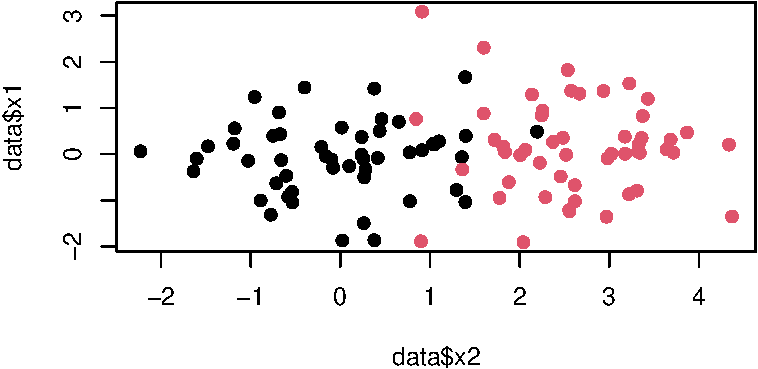
\includegraphics{lista-5_files/figure-pdf/unnamed-chunk-18-1.pdf}

~

\subsubsection{Item b)}\label{item-b-3}

Compute the cross-validation error rates for support vector classifiers
with a range of cost values. How many training observations are
misclassified for each value of cost considered, and how does this
relate to the cross-validation errors obtained?

\begin{center}\rule{0.5\linewidth}{0.5pt}\end{center}

~

Computando os erros de validação cruzada para os valores de custo 0.1,
1, 10 e 100. Pela utilização da função tune() o melhor valor de custo é
de 100 visto que é o que tem o menor erro de validação cruzada.

\begin{Shaded}
\begin{Highlighting}[]
\NormalTok{tune.out }\OtherTok{\textless{}{-}} \FunctionTok{tune}\NormalTok{(svm ,y }\SpecialCharTok{\textasciitilde{}}\NormalTok{ . , }\AttributeTok{data =}\NormalTok{ data , }\AttributeTok{kernel =} \StringTok{"linear"}\NormalTok{,}
                 \AttributeTok{ranges =} \FunctionTok{list}\NormalTok{(}\AttributeTok{cost =} \FunctionTok{c}\NormalTok{( }\FloatTok{0.1}\NormalTok{, }\DecValTok{1}\NormalTok{, }\DecValTok{10}\NormalTok{, }\DecValTok{100}\NormalTok{,}\DecValTok{150}\NormalTok{)),}\AttributeTok{scale=}\ConstantTok{FALSE}\NormalTok{)}
\FunctionTok{summary}\NormalTok{(tune.out)}
\end{Highlighting}
\end{Shaded}

\begin{verbatim}

Parameter tuning of 'svm':

- sampling method: 10-fold cross validation 

- best parameters:
 cost
   10

- best performance: 0.05909091 

- Detailed performance results:
   cost      error dispersion
1   0.1 0.09818182 0.09229250
2   1.0 0.06909091 0.08200876
3  10.0 0.05909091 0.08389617
4 100.0 0.05909091 0.08389617
5 150.0 0.05909091 0.08389617
\end{verbatim}

A seguir seram ajustados modelos para cada valor de custo e a matriz de
confusão para cada modelo nos dados de treino.

\paragraph{valor 0.1}\label{valor-0.1}

Errou 8 observações.

\begin{Shaded}
\begin{Highlighting}[]
\NormalTok{modkernel1 }\OtherTok{\textless{}{-}} \FunctionTok{svm}\NormalTok{(y }\SpecialCharTok{\textasciitilde{}}\NormalTok{ ., }\AttributeTok{data=}\NormalTok{data, }\AttributeTok{kernel=}\StringTok{"linear"}\NormalTok{,}\AttributeTok{cost=}\FloatTok{0.1}\NormalTok{)}
  
\NormalTok{pred1}\OtherTok{\textless{}{-}}\FunctionTok{predict}\NormalTok{(modkernel1,data)}
\FunctionTok{confusionMatrix}\NormalTok{(pred1,data}\SpecialCharTok{$}\NormalTok{y)}
\end{Highlighting}
\end{Shaded}

\begin{verbatim}
Confusion Matrix and Statistics

          Reference
Prediction  A  B
         A 47  4
         B  4 47
                                          
               Accuracy : 0.9216          
                 95% CI : (0.8513, 0.9655)
    No Information Rate : 0.5             
    P-Value [Acc > NIR] : <2e-16          
                                          
                  Kappa : 0.8431          
                                          
 Mcnemar's Test P-Value : 1               
                                          
            Sensitivity : 0.9216          
            Specificity : 0.9216          
         Pos Pred Value : 0.9216          
         Neg Pred Value : 0.9216          
             Prevalence : 0.5000          
         Detection Rate : 0.4608          
   Detection Prevalence : 0.5000          
      Balanced Accuracy : 0.9216          
                                          
       'Positive' Class : A               
                                          
\end{verbatim}

\paragraph{valor 1}\label{valor-1}

Errou 7 observações.

\begin{Shaded}
\begin{Highlighting}[]
\NormalTok{modkernel2 }\OtherTok{\textless{}{-}} \FunctionTok{svm}\NormalTok{(y }\SpecialCharTok{\textasciitilde{}}\NormalTok{ ., }\AttributeTok{data=}\NormalTok{data, }\AttributeTok{kernel=}\StringTok{"linear"}\NormalTok{,}\AttributeTok{cost=}\DecValTok{1}\NormalTok{)}

\NormalTok{pred2}\OtherTok{\textless{}{-}}\FunctionTok{predict}\NormalTok{(modkernel2,data)}
\FunctionTok{confusionMatrix}\NormalTok{(pred2,data}\SpecialCharTok{$}\NormalTok{y)}
\end{Highlighting}
\end{Shaded}

\begin{verbatim}
Confusion Matrix and Statistics

          Reference
Prediction  A  B
         A 48  4
         B  3 47
                                         
               Accuracy : 0.9314         
                 95% CI : (0.8637, 0.972)
    No Information Rate : 0.5            
    P-Value [Acc > NIR] : <2e-16         
                                         
                  Kappa : 0.8627         
                                         
 Mcnemar's Test P-Value : 1              
                                         
            Sensitivity : 0.9412         
            Specificity : 0.9216         
         Pos Pred Value : 0.9231         
         Neg Pred Value : 0.9400         
             Prevalence : 0.5000         
         Detection Rate : 0.4706         
   Detection Prevalence : 0.5098         
      Balanced Accuracy : 0.9314         
                                         
       'Positive' Class : A              
                                         
\end{verbatim}

\paragraph{valor 10}\label{valor-10}

Errou 7 observações.

\begin{Shaded}
\begin{Highlighting}[]
\NormalTok{modkernel3 }\OtherTok{\textless{}{-}} \FunctionTok{svm}\NormalTok{(y }\SpecialCharTok{\textasciitilde{}}\NormalTok{ ., }\AttributeTok{data=}\NormalTok{data, }\AttributeTok{kernel=}\StringTok{"linear"}\NormalTok{,}\AttributeTok{cost=}\DecValTok{10}\NormalTok{)}

\NormalTok{pred3}\OtherTok{\textless{}{-}}\FunctionTok{predict}\NormalTok{(modkernel3,data)}
\FunctionTok{confusionMatrix}\NormalTok{(pred3,data}\SpecialCharTok{$}\NormalTok{y)}
\end{Highlighting}
\end{Shaded}

\begin{verbatim}
Confusion Matrix and Statistics

          Reference
Prediction  A  B
         A 48  4
         B  3 47
                                         
               Accuracy : 0.9314         
                 95% CI : (0.8637, 0.972)
    No Information Rate : 0.5            
    P-Value [Acc > NIR] : <2e-16         
                                         
                  Kappa : 0.8627         
                                         
 Mcnemar's Test P-Value : 1              
                                         
            Sensitivity : 0.9412         
            Specificity : 0.9216         
         Pos Pred Value : 0.9231         
         Neg Pred Value : 0.9400         
             Prevalence : 0.5000         
         Detection Rate : 0.4706         
   Detection Prevalence : 0.5098         
      Balanced Accuracy : 0.9314         
                                         
       'Positive' Class : A              
                                         
\end{verbatim}

\paragraph{Valor 100}\label{valor-100}

Errou 6 observações.

\begin{Shaded}
\begin{Highlighting}[]
\NormalTok{modkernel4 }\OtherTok{\textless{}{-}} \FunctionTok{svm}\NormalTok{(y }\SpecialCharTok{\textasciitilde{}}\NormalTok{ ., }\AttributeTok{data=}\NormalTok{data, }\AttributeTok{kernel=}\StringTok{"linear"}\NormalTok{,}\AttributeTok{cost=}\DecValTok{100}\NormalTok{)}

\NormalTok{pred4}\OtherTok{\textless{}{-}}\FunctionTok{predict}\NormalTok{(modkernel4,data)}
\FunctionTok{confusionMatrix}\NormalTok{(pred4,data}\SpecialCharTok{$}\NormalTok{y)}
\end{Highlighting}
\end{Shaded}

\begin{verbatim}
Confusion Matrix and Statistics

          Reference
Prediction  A  B
         A 49  4
         B  2 47
                                          
               Accuracy : 0.9412          
                 95% CI : (0.8764, 0.9781)
    No Information Rate : 0.5             
    P-Value [Acc > NIR] : <2e-16          
                                          
                  Kappa : 0.8824          
                                          
 Mcnemar's Test P-Value : 0.6831          
                                          
            Sensitivity : 0.9608          
            Specificity : 0.9216          
         Pos Pred Value : 0.9245          
         Neg Pred Value : 0.9592          
             Prevalence : 0.5000          
         Detection Rate : 0.4804          
   Detection Prevalence : 0.5196          
      Balanced Accuracy : 0.9412          
                                          
       'Positive' Class : A               
                                          
\end{verbatim}

\paragraph{Valor 150}\label{valor-150}

\begin{Shaded}
\begin{Highlighting}[]
\NormalTok{modkernel5 }\OtherTok{\textless{}{-}} \FunctionTok{svm}\NormalTok{(y }\SpecialCharTok{\textasciitilde{}}\NormalTok{ ., }\AttributeTok{data=}\NormalTok{data, }\AttributeTok{kernel=}\StringTok{"linear"}\NormalTok{,}\AttributeTok{cost=}\DecValTok{150}\NormalTok{)}

\NormalTok{pred5}\OtherTok{\textless{}{-}}\FunctionTok{predict}\NormalTok{(modkernel5,data)}
\FunctionTok{confusionMatrix}\NormalTok{(pred5,data}\SpecialCharTok{$}\NormalTok{y)}
\end{Highlighting}
\end{Shaded}

\begin{verbatim}
Confusion Matrix and Statistics

          Reference
Prediction  A  B
         A 49  4
         B  2 47
                                          
               Accuracy : 0.9412          
                 95% CI : (0.8764, 0.9781)
    No Information Rate : 0.5             
    P-Value [Acc > NIR] : <2e-16          
                                          
                  Kappa : 0.8824          
                                          
 Mcnemar's Test P-Value : 0.6831          
                                          
            Sensitivity : 0.9608          
            Specificity : 0.9216          
         Pos Pred Value : 0.9245          
         Neg Pred Value : 0.9592          
             Prevalence : 0.5000          
         Detection Rate : 0.4804          
   Detection Prevalence : 0.5196          
      Balanced Accuracy : 0.9412          
                                          
       'Positive' Class : A               
                                          
\end{verbatim}

Como indicado na tabela de erros de validação cruzada o aumento de custo
a partir do valor de custo 10, se torna redundante, classificando no
máximo 1 observação a mais de forma certa.

~

\subsubsection{Item c)}\label{item-c-2}

Generate an appropriate test data set, and compute the test errors
corresponding to each of the values of cost considered. Which value of
cost leads to the fewest test errors, and how does this compare to the
values of cost that yield the fewest training errors and the fewest
cross-validation errors?

\begin{center}\rule{0.5\linewidth}{0.5pt}\end{center}

~

Criando 20 amostras de teste que se asemelham aos dados de treinamento

\begin{Shaded}
\begin{Highlighting}[]
\NormalTok{datateste }\OtherTok{\textless{}{-}} \FunctionTok{data.frame}\NormalTok{(}
  \AttributeTok{x1 =} \FunctionTok{rnorm}\NormalTok{(}\DecValTok{20}\NormalTok{),}
  \AttributeTok{x2 =} \FunctionTok{rnorm}\NormalTok{(}\DecValTok{20}\NormalTok{),}
  \AttributeTok{y =} \FunctionTok{factor}\NormalTok{(}\FunctionTok{rep}\NormalTok{(}\FunctionTok{c}\NormalTok{(}\StringTok{\textquotesingle{}A\textquotesingle{}}\NormalTok{, }\StringTok{\textquotesingle{}B\textquotesingle{}}\NormalTok{), }\AttributeTok{each=}\DecValTok{10}\NormalTok{))}
\NormalTok{)}
\NormalTok{datateste}\SpecialCharTok{$}\NormalTok{x2[}\DecValTok{11}\SpecialCharTok{:}\DecValTok{20}\NormalTok{]}\OtherTok{\textless{}{-}}\NormalTok{datateste}\SpecialCharTok{$}\NormalTok{x2[}\DecValTok{11}\SpecialCharTok{:}\DecValTok{20}\NormalTok{]}\SpecialCharTok{+}\FloatTok{2.2}
\FunctionTok{plot}\NormalTok{(datateste}\SpecialCharTok{$}\NormalTok{x1, datateste}\SpecialCharTok{$}\NormalTok{x2, }\AttributeTok{col=}\NormalTok{datateste}\SpecialCharTok{$}\NormalTok{y, }\AttributeTok{pch=}\DecValTok{19}\NormalTok{)}
\end{Highlighting}
\end{Shaded}

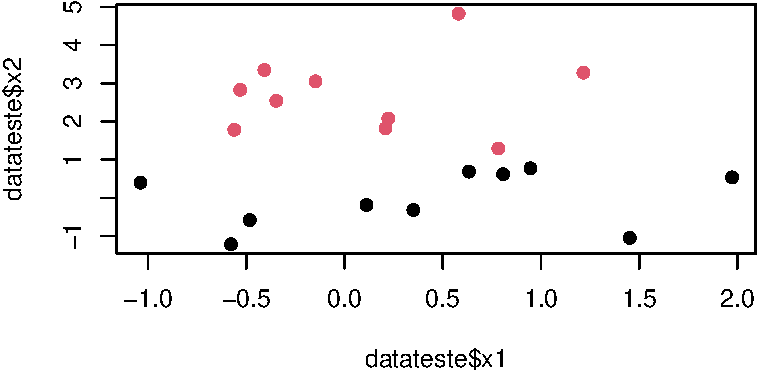
\includegraphics{lista-5_files/figure-pdf/unnamed-chunk-25-1.pdf}

A partir da função tune() é indicado que para os dados de teste o custo
que melhor otimiza o modelo é 1

\begin{Shaded}
\begin{Highlighting}[]
\NormalTok{tune.out1 }\OtherTok{\textless{}{-}} \FunctionTok{tune}\NormalTok{(svm ,y }\SpecialCharTok{\textasciitilde{}}\NormalTok{ . , }\AttributeTok{data =}\NormalTok{ data , }\AttributeTok{kernel =} \StringTok{"linear"}\NormalTok{,}
                 \AttributeTok{ranges =} \FunctionTok{list}\NormalTok{(}\AttributeTok{cost =} \FunctionTok{c}\NormalTok{( }\FloatTok{0.1}\NormalTok{, }\DecValTok{1}\NormalTok{, }\DecValTok{10}\NormalTok{, }\DecValTok{100}\NormalTok{,}\DecValTok{150}\NormalTok{)),}\AttributeTok{scale=}\ConstantTok{FALSE}\NormalTok{)}
\FunctionTok{summary}\NormalTok{(tune.out1)}
\end{Highlighting}
\end{Shaded}

\begin{verbatim}

Parameter tuning of 'svm':

- sampling method: 10-fold cross validation 

- best parameters:
 cost
  100

- best performance: 0.06727273 

- Detailed performance results:
   cost      error dispersion
1   0.1 0.08636364 0.09312945
2   1.0 0.07727273 0.08476728
3  10.0 0.07727273 0.09699337
4 100.0 0.06727273 0.09951212
5 150.0 0.06727273 0.09951212
\end{verbatim}

\begin{Shaded}
\begin{Highlighting}[]
\NormalTok{bestmodelteste}\OtherTok{\textless{}{-}}\NormalTok{tune.out1}\SpecialCharTok{$}\NormalTok{best.model}
\NormalTok{predteste}\OtherTok{\textless{}{-}}\FunctionTok{predict}\NormalTok{(bestmodelteste,datateste)}
\FunctionTok{confusionMatrix}\NormalTok{(predteste,datateste}\SpecialCharTok{$}\NormalTok{y)}
\end{Highlighting}
\end{Shaded}

\begin{verbatim}
Confusion Matrix and Statistics

          Reference
Prediction  A  B
         A 10  1
         B  0  9
                                          
               Accuracy : 0.95            
                 95% CI : (0.7513, 0.9987)
    No Information Rate : 0.5             
    P-Value [Acc > NIR] : 2.003e-05       
                                          
                  Kappa : 0.9             
                                          
 Mcnemar's Test P-Value : 1               
                                          
            Sensitivity : 1.0000          
            Specificity : 0.9000          
         Pos Pred Value : 0.9091          
         Neg Pred Value : 1.0000          
             Prevalence : 0.5000          
         Detection Rate : 0.5000          
   Detection Prevalence : 0.5500          
      Balanced Accuracy : 0.9500          
                                          
       'Positive' Class : A               
                                          
\end{verbatim}

\subsubsection{Item d)}\label{item-d-2}

Discuss your results.

\begin{center}\rule{0.5\linewidth}{0.5pt}\end{center}

As questões acima mostram que a escolha do valor de custo deve ser feito
com cuidado, de forma a não usar valores muito altos de custo ou seja
mais restritos para a divisão de classes visto que a partir de um certo
valor não ha mais ganho no aumento do valor do custo para a
classificação do modelo.

~

\subsection{Questão 7}\label{questuxe3o-7}

In this problem, you will use support vector approaches in order to
predict whether a given car gets high or low gas mileage based on the
\texttt{ISLR::Auto} data set.

\subsubsection{Item a)}\label{item-a-4}

Create a binary variable that takes on a 1 for cars with gas mileage
above the median, and a 0 for cars with gas mileage below the median.

\begin{center}\rule{0.5\linewidth}{0.5pt}\end{center}

~

\begin{Shaded}
\begin{Highlighting}[]
\NormalTok{auto }\OtherTok{\textless{}{-}}\NormalTok{ ISLR}\SpecialCharTok{::}\NormalTok{Auto }\SpecialCharTok{\%\textgreater{}\%}
  \FunctionTok{mutate}\NormalTok{(}\AttributeTok{mpg01 =} \FunctionTok{if\_else}\NormalTok{(mpg }\SpecialCharTok{\textgreater{}} \FunctionTok{median}\NormalTok{(mpg), }\DecValTok{1}\NormalTok{, }\DecValTok{0}\NormalTok{))}
\end{Highlighting}
\end{Shaded}

~

\subsubsection{Item b)}\label{item-b-4}

Fit a support vector classifier to the data with various values of
\texttt{cost}, in order to predict whether a car gets high or low gas
mileage. Report the cross-validation errors associated with different
values of this parameter. Comment on your results. Note you will need to
fit the classifier without the gas mileage variable to produce sensible
results.

\begin{center}\rule{0.5\linewidth}{0.5pt}\end{center}

~

A seguir é ajustado um classificador linear com valores de custo iguals
a 0.1, 1, 10, 100 e 1000 e é usada validação cruzada com 10 folds para
avaliar o desempenho do modelo. Isto é, a base de dados é particionada
em 10 pedaços e o modelo é ajustado 10 vezes, cada vez utilizando 9
pedaços para treinamento e 1 para teste. O erro de classificação é
calculado para cada ajuste e a média dos erros é reportada.

De acordo com os resultados do \texttt{summary()}, o modelo com cursto
igual a 1 apresentou os melhores resultados, com 9,5\% de erro.

~

\begin{Shaded}
\begin{Highlighting}[]
\NormalTok{auto\_nompg }\OtherTok{\textless{}{-}}\NormalTok{ auto }\SpecialCharTok{\%\textgreater{}\%} \FunctionTok{select}\NormalTok{(}\SpecialCharTok{{-}}\NormalTok{mpg)}

\FunctionTok{set.seed}\NormalTok{ (}\DecValTok{1}\NormalTok{)}
\NormalTok{tune.svc }\OtherTok{\textless{}{-}} \FunctionTok{tune}\NormalTok{(svm, mpg01 }\SpecialCharTok{\textasciitilde{}}\NormalTok{ ., }\AttributeTok{data =}\NormalTok{ auto\_nompg,}
                   \AttributeTok{kernel =} \StringTok{"linear"}\NormalTok{,}
                   \AttributeTok{ranges =} \FunctionTok{list}\NormalTok{(}
                     \AttributeTok{cost =} \FunctionTok{c}\NormalTok{(}\FloatTok{0.1}\NormalTok{, }\DecValTok{1}\NormalTok{, }\DecValTok{10}\NormalTok{, }\DecValTok{100}\NormalTok{, }\DecValTok{1000}\NormalTok{)}
\NormalTok{                   )}
\NormalTok{)}

\FunctionTok{summary}\NormalTok{(tune.svc)}
\end{Highlighting}
\end{Shaded}

\begin{verbatim}

Parameter tuning of 'svm':

- sampling method: 10-fold cross validation 

- best parameters:
 cost
    1

- best performance: 0.09603609 

- Detailed performance results:
   cost      error dispersion
1 1e-01 0.10227373 0.03634911
2 1e+00 0.09603609 0.03666741
3 1e+01 0.10531309 0.03683207
4 1e+02 0.12079079 0.03864160
5 1e+03 0.12724775 0.03878303
\end{verbatim}

~

\subsubsection{Item c)}\label{item-c-3}

Now repeat (b), this time using SVMs with radial and polynomial basis
kernels, with different values of \texttt{gamma} and \texttt{degree} and
cost. Comment on your results.

\begin{center}\rule{0.5\linewidth}{0.5pt}\end{center}

~

A seguir são ajustados modelos SVM com kernel polinomial e radial,
variando os valores de \texttt{cost} e \texttt{degree} para o polinomial
e \texttt{cost} e \texttt{gamma} para o radial.

~

\begin{Shaded}
\begin{Highlighting}[]
\FunctionTok{set.seed}\NormalTok{ (}\DecValTok{1}\NormalTok{)}
\NormalTok{tune.svpoly }\OtherTok{\textless{}{-}} \FunctionTok{tune}\NormalTok{(svm, mpg01 }\SpecialCharTok{\textasciitilde{}}\NormalTok{ ., }\AttributeTok{data =}\NormalTok{ auto\_nompg,}
                   \AttributeTok{kernel =} \StringTok{"polynomial"}\NormalTok{,}
                   \AttributeTok{ranges =} \FunctionTok{list}\NormalTok{(}
                     \AttributeTok{cost =} \FunctionTok{c}\NormalTok{(}\FloatTok{0.1}\NormalTok{, }\DecValTok{1}\NormalTok{, }\DecValTok{10}\NormalTok{, }\DecValTok{100}\NormalTok{, }\DecValTok{1000}\NormalTok{),}
                     \AttributeTok{degree =} \FunctionTok{c}\NormalTok{(}\DecValTok{2}\NormalTok{, }\DecValTok{3}\NormalTok{, }\DecValTok{4}\NormalTok{, }\DecValTok{5}\NormalTok{)}
\NormalTok{                   )}
\NormalTok{)}
\end{Highlighting}
\end{Shaded}

\begin{Shaded}
\begin{Highlighting}[]
\FunctionTok{set.seed}\NormalTok{ (}\DecValTok{1}\NormalTok{)}
\NormalTok{tune.svradial }\OtherTok{\textless{}{-}} \FunctionTok{tune}\NormalTok{(svm, mpg01 }\SpecialCharTok{\textasciitilde{}}\NormalTok{ ., }\AttributeTok{data =}\NormalTok{ auto\_nompg,}
                   \AttributeTok{kernel =} \StringTok{"radial"}\NormalTok{,}
                   \AttributeTok{ranges =} \FunctionTok{list}\NormalTok{(}
                     \AttributeTok{cost =} \FunctionTok{c}\NormalTok{(}\FloatTok{0.1}\NormalTok{, }\DecValTok{1}\NormalTok{, }\DecValTok{10}\NormalTok{, }\DecValTok{100}\NormalTok{, }\DecValTok{1000}\NormalTok{),}
                     \AttributeTok{gamma =} \FunctionTok{c}\NormalTok{(}\FloatTok{0.5}\NormalTok{, }\DecValTok{1}\NormalTok{, }\DecValTok{2}\NormalTok{, }\DecValTok{3}\NormalTok{, }\DecValTok{4}\NormalTok{)}
\NormalTok{                   )}
\NormalTok{)}
\end{Highlighting}
\end{Shaded}

~

Os resultados para os modelos ajustados com kernel polinomial e radial
são apresentados a seguir. O modelo polinomial via de regra apresenta
resultados precários. O melhor resultado, com 15\% de erros, ocorre com
um polinômio de grau 2 e erro igual a 1000. O modelo radial, por outro
lado, apresenta resultados melhores, com erro de 6,5\% para custo igual
a 1 e \(\gamma\) igual a 0.5. Conclui-se que o modelo radial é o mais
indicado, considerando apenas as simulações.

~

\begin{Shaded}
\begin{Highlighting}[]
\FunctionTok{summary}\NormalTok{(tune.svpoly)}
\end{Highlighting}
\end{Shaded}

\begin{verbatim}

Parameter tuning of 'svm':

- sampling method: 10-fold cross validation 

- best parameters:
 cost degree
 1000      2

- best performance: 0.1594745 

- Detailed performance results:
    cost degree     error dispersion
1  1e-01      2 0.4960905 0.03974005
2  1e+00      2 0.4752293 0.04525479
3  1e+01      2 0.3375643 0.08311313
4  1e+02      2 0.2548390 0.07343884
5  1e+03      2 0.1594745 0.05452093
6  1e-01      3 0.4978768 0.03935396
7  1e+00      3 0.4924827 0.03986701
8  1e+01      3 0.4418838 0.04913560
9  1e+02      3 0.2465708 0.05122197
10 1e+03      3 0.1683651 0.03763027
11 1e-01      4 0.4984602 0.03930559
12 1e+00      4 0.4983427 0.03933257
13 1e+01      4 0.4971505 0.03961089
14 1e+02      4 0.4855727 0.04370976
15 1e+03      4 0.3998639 0.09315902
16 1e-01      5 0.4984718 0.03930295
17 1e+00      5 0.4984585 0.03930611
18 1e+01      5 0.4983260 0.03933773
19 1e+02      5 0.4969797 0.03965863
20 1e+03      5 0.4838647 0.04389044
\end{verbatim}

\begin{Shaded}
\begin{Highlighting}[]
\FunctionTok{summary}\NormalTok{(tune.svradial)}
\end{Highlighting}
\end{Shaded}

\begin{verbatim}

Parameter tuning of 'svm':

- sampling method: 10-fold cross validation 

- best parameters:
 cost gamma
    1   0.5

- best performance: 0.0657775 

- Detailed performance results:
    cost gamma      error  dispersion
1  1e-01   0.5 0.08548406 0.021104890
2  1e+00   0.5 0.06577750 0.026197728
3  1e+01   0.5 0.07304343 0.027869128
4  1e+02   0.5 0.07667563 0.027824986
5  1e+03   0.5 0.07667563 0.027824986
6  1e-01   1.0 0.27951125 0.036343997
7  1e+00   1.0 0.09918732 0.020523476
8  1e+01   1.0 0.10442706 0.020690277
9  1e+02   1.0 0.10442540 0.020692046
10 1e+03   1.0 0.10442540 0.020692046
11 1e-01   2.0 0.42047779 0.044561140
12 1e+00   2.0 0.20409900 0.013765977
13 1e+01   2.0 0.20506214 0.013269495
14 1e+02   2.0 0.20506214 0.013269495
15 1e+03   2.0 0.20506214 0.013269495
16 1e-01   3.0 0.43453116 0.043273628
17 1e+00   3.0 0.23107129 0.010987668
18 1e+01   3.0 0.23126372 0.010794330
19 1e+02   3.0 0.23126372 0.010794330
20 1e+03   3.0 0.23126372 0.010794330
21 1e-01   4.0 0.43894907 0.041927995
22 1e+00   4.0 0.23592639 0.009193937
23 1e+01   4.0 0.23597971 0.009134275
24 1e+02   4.0 0.23597971 0.009134275
25 1e+03   4.0 0.23597971 0.009134275
\end{verbatim}

~

\subsubsection{Item d)}\label{item-d-3}

Make some plots to back up your assertions in (b) and (c).

\begin{center}\rule{0.5\linewidth}{0.5pt}\end{center}

~

A seguir, para comparar os modelos de forma sintética, são comparadas as
curvas ROC para os melhores modelos de cada categoria. O que se pode
observar na Figura~\ref{fig-q7d} é uma confirmação de que o modelo
polinomial tem um desempenho consideravelmente pior que os demais.
Enquanto o modelo radial parece apresentar quase desempenho perfeito ---
o que pode ser um indicador de overfitting --- o modelo linear apresenta
um desempenho comparável a este e, por isso, pode apresentar uma
flexibilidade maior para classificação de novas observações.

~

\begin{Shaded}
\begin{Highlighting}[]
\NormalTok{fit\_svc }\OtherTok{\textless{}{-}} \FunctionTok{attributes}\NormalTok{(}\FunctionTok{predict}\NormalTok{(tune.svc}\SpecialCharTok{$}\NormalTok{best.model , auto\_nompg, }\AttributeTok{decision.values =}\NormalTok{ T))}\SpecialCharTok{$}\NormalTok{decision.values}

\NormalTok{fit\_svpoly }\OtherTok{\textless{}{-}} \FunctionTok{attributes}\NormalTok{(}\FunctionTok{predict}\NormalTok{(tune.svpoly}\SpecialCharTok{$}\NormalTok{best.model , auto\_nompg, }\AttributeTok{decision.values =}\NormalTok{ T))}\SpecialCharTok{$}\NormalTok{decision.values}

\NormalTok{fit\_svradial }\OtherTok{\textless{}{-}} \FunctionTok{attributes}\NormalTok{(}\FunctionTok{predict}\NormalTok{(tune.svradial}\SpecialCharTok{$}\NormalTok{best.model , auto\_nompg, }\AttributeTok{decision.values =}\NormalTok{ T))}\SpecialCharTok{$}\NormalTok{decision.values}

\FunctionTok{rocplot}\NormalTok{(fit\_svc , auto\_nompg}\SpecialCharTok{$}\NormalTok{mpg01, }\AttributeTok{col =} \StringTok{"red"}\NormalTok{)}
\FunctionTok{rocplot}\NormalTok{(fit\_svpoly , auto\_nompg}\SpecialCharTok{$}\NormalTok{mpg01, }\AttributeTok{add =}\NormalTok{ T, }\AttributeTok{col =} \StringTok{"blue"}\NormalTok{)}
\FunctionTok{rocplot}\NormalTok{(fit\_svradial , auto\_nompg}\SpecialCharTok{$}\NormalTok{mpg01, }\AttributeTok{add =}\NormalTok{ T, }\AttributeTok{col =} \StringTok{"green"}\NormalTok{)}
\FunctionTok{legend}\NormalTok{(}\StringTok{"bottomright"}\NormalTok{, }\AttributeTok{legend =} \FunctionTok{c}\NormalTok{(}\StringTok{"Linear"}\NormalTok{, }\StringTok{"Poli."}\NormalTok{, }\StringTok{"Radial"}\NormalTok{), }\AttributeTok{col =} \FunctionTok{c}\NormalTok{(}\StringTok{"red"}\NormalTok{, }\StringTok{"blue"}\NormalTok{, }\StringTok{"green"}\NormalTok{), }\AttributeTok{pch =} \DecValTok{16}\NormalTok{)}
\end{Highlighting}
\end{Shaded}

\begin{figure}[H]

\centering{

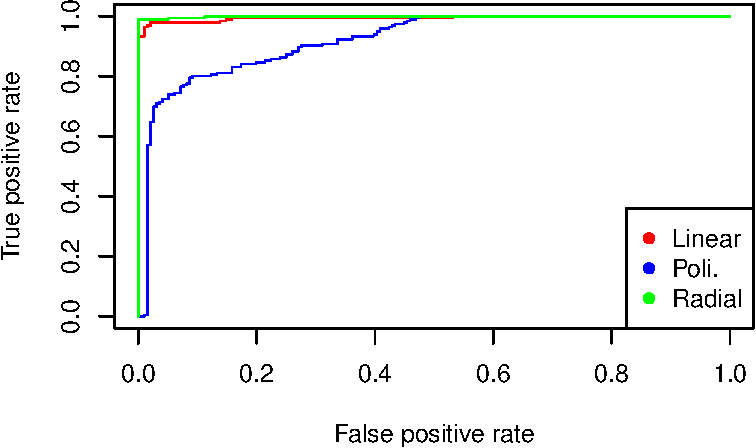
\includegraphics{lista-5_files/figure-pdf/fig-q7d-1.pdf}

}

\caption{\label{fig-q7d}Curvas ROC para os modelos ajustados com SVMs}

\end{figure}%

~ ~

\section{Questão 13}\label{questuxe3o-13}

Escolha uma linguagem de programação (\texttt{R}, \texttt{Python},
\texttt{SAS}, \texttt{Matlab}, \texttt{Julia}) e apresente um exemplo de
classificação com SVM utilizando Kernel Linear e outro utilizando Kernel
não Linear.

\begin{center}\rule{0.5\linewidth}{0.5pt}\end{center}

~

No \texttt{SAS}, a função implementada para realizar análises utilizando
algoritmos de suporte vetorial (SVM) é o \texttt{PROC\ HPSVM}. Essa
função permite o uso de kernels lineares e não lineares nos dados de
treinamento. O \texttt{PROC\ HPSVM} executa o algoritmo SVM de alta
performance, possibilitando sua execução em computação paralela tanto em
uma única máquina quanto em múltiplas máquinas.\footnote{\url{https://documentation.sas.com/doc/en/emhpprcref/14.2/emhpprcref_hpsvm_overview.htm}}

Utilizando o exemplo fornecido na documentação do \texttt{SAS} com um
kernel linear, vamos ajustar um modelo utilizando um banco de dados
chamado \texttt{SAMPSIO.DMAGECR}, um banco de dados de referência que
traz informações sobre risco de crédito\footnote{\url{https://support.sas.com/documentation/cdl/en/emgs/59885/HTML/default/viewer.htm\#a001026918.htm}}.
Esse banco de dados faz parte da biblioteca \texttt{SAMPSIO} e contém
1.000 observações, cada uma com informações detalhadas sobre os
requerentes. O banco inclui a classificação do indivíduo como GOOD ou
BAD em uma variável denominada GOOD\_BAD, além de outras variáveis como
histórico de crédito, duração do empréstimo, entre outras.

A tabela `Matriz de Classificação' mostra que, entre as 1.000
observações totais, 700 são classificadas como boas e 300 como ruins. O
número de observações BOAS corretamente previstas é 626, e o número de
observações RUINS corretamente previstas é 158.

\begin{center}
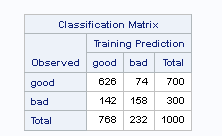
\includegraphics{tabela_classification1.png}
\end{center}

Assim, a precisão do modelo é de 78,4\%, conforme indicado na tabela
`Estatísticas de Ajuste'.

\begin{center}
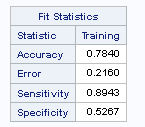
\includegraphics{tabela_fit1.png}
\end{center}

Um modelo relativamente bom significa que a taxa de erro de
classificação é baixa, enquanto a sensibilidade e a especificidade são
altas. Com o PROC HPSVM, é possível ajustar os parâmetros de treinamento
e usar diferentes kernels para obter um modelo melhor. O padrão do
procedimento usa o kernel linear conforme especificado:

\begin{align} 
  k(x_1, x_2) = \langle x_1, x_2 \rangle, 
\end{align}

onde \(x_1\) e \(x_2\) são dois vetores e
\(\langle \cdot, \cdot \rangle\) é o produto interno. Para alterar o
tipo de kernel utilizado, basta definir o argumento KERNEL,
especificando o tipo de kernel e quaisquer parâmetros associados.
Definindo o kernel como polinomial:

\begin{align}
  k(x_1, x_2) = \left(\langle x_1, x_2 \rangle + 1 \right)^p,
\end{align}

onde \(p\) é o grau do polinômio, obtém-se o resultado:

\begin{center}
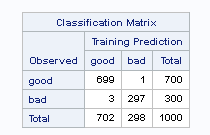
\includegraphics{tabela_classification.png}
\end{center}

A matriz de classificação mostra que o número de observações BOAS
corretamente previstas é 699, e o número de observações RUINS
corretamente previstas é 297. Assim, a precisão do modelo é de 99,6\%,
conforme indicado na tabela `Estatísticas de Ajuste', mostrando que o
uso do kernel polinomial é mais acurado, nesse caso.

\begin{center}
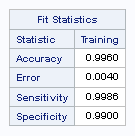
\includegraphics{tabela_fit.png}
\end{center}

O código a seguir foi utilizado para gerar os resultados desta questão:

\begin{Shaded}
\begin{Highlighting}[]
\NormalTok{proc freq data }\OtherTok{=}\NormalTok{ sampsio.dmagecr;}
\NormalTok{ tables GOOD\_BAD;}
\NormalTok{ run;}
 
 
\NormalTok{ proc hpsvm data}\OtherTok{=}\NormalTok{sampsio.dmagecr;}
\NormalTok{     input checking history purpose savings employed marital coapp}
\NormalTok{           property other job housing telephon foreign}\SpecialCharTok{/}\NormalTok{level}\OtherTok{=}\NormalTok{nominal;}
\NormalTok{     input duration amount installp resident existcr depends age}\SpecialCharTok{/}\NormalTok{level}\OtherTok{=}\NormalTok{interval;}
\NormalTok{     target good\_bad;}
\NormalTok{     KERNEL LINEAR;}
\NormalTok{ run;}

\SpecialCharTok{/}\ErrorTok{*}\NormalTok{ Ajustando o modelo SVM }
\NormalTok{proc hpsvm data}\OtherTok{=}\NormalTok{sampsio.dmagecr;}
\NormalTok{    input checking history purpose savings employed marital coapp}
\NormalTok{          property other job housing telephon foreign }\SpecialCharTok{/}\NormalTok{ level}\OtherTok{=}\NormalTok{nominal;}
\NormalTok{    input duration amount installp resident existcr depends age }\SpecialCharTok{/}\NormalTok{ level}\OtherTok{=}\NormalTok{interval;}
\NormalTok{    target good\_bad }\SpecialCharTok{/}\NormalTok{ level}\OtherTok{=}\NormalTok{nominal;}
\NormalTok{    id duration amount;}
\NormalTok{    savestate rstore}\OtherTok{=}\NormalTok{work.svm\_model;}
\NormalTok{run;}

\NormalTok{Aplicando o modelo ajustado aos dados e salvando os resultados }
\NormalTok{proc astore;}
\NormalTok{    score data}\OtherTok{=}\NormalTok{sampsio.dmagecr out}\OtherTok{=}\NormalTok{svm\_results rstore}\OtherTok{=}\NormalTok{work.svm\_model;}
\NormalTok{run;}

\NormalTok{Gerando um gráfico de dispersão para visualizar a distribuição das classes previstas }
\NormalTok{proc sgplot data}\OtherTok{=}\NormalTok{svm\_results;}
\NormalTok{    scatter x}\OtherTok{=}\NormalTok{amount y}\OtherTok{=}\NormalTok{duration }\SpecialCharTok{/}\NormalTok{ group}\OtherTok{=}\NormalTok{P\_good\_bad;}
\NormalTok{    xaxis label}\OtherTok{=}\StringTok{"Amount"}\NormalTok{;}
\NormalTok{    yaxis label}\OtherTok{=}\StringTok{"Duration"}\NormalTok{;}
\NormalTok{    title }\StringTok{"Gráfico de Dispersão das Classes Previstas pelo Modelo SVM"}\NormalTok{;}
\NormalTok{run;}\SpecialCharTok{*}\ErrorTok{/}

\NormalTok{ proc hpsvm data}\OtherTok{=}\NormalTok{sampsio.dmagecr;}
\NormalTok{     input checking history purpose savings employed marital coapp}
\NormalTok{           property other job housing telephon foreign}\SpecialCharTok{/}\NormalTok{level}\OtherTok{=}\NormalTok{nominal;}
\NormalTok{     input duration amount installp resident existcr depends age}\SpecialCharTok{/}\NormalTok{level}\OtherTok{=}\NormalTok{interval;}
\NormalTok{     target good\_bad;}
\NormalTok{     KERNEL POLYNOM;}
\NormalTok{ run;}
\end{Highlighting}
\end{Shaded}




\end{document}
